\documentclass{article}
\usepackage{graphicx}
\usepackage{hyperref}
\usepackage{amsthm}
\usepackage{amsmath}
\usepackage{amssymb}
\usepackage{listings}
\usepackage{algorithm}
\usepackage{algpseudocode}

\lstset{basicstyle=\ttfamily}

\newtheorem{definition}{Definition}

\title{\huge{\textit{Foundations of \\ Artificial Intelligence}}}
\author{Fabio Vokrri}
\date{October 2024}

\begin{document}

\maketitle
\newpage
\tableofcontents

\newpage
\section{Introduction}
There isn't a single definition of Artificial Intelligence: some define intelligence in terms of fidelity to human performance, while others prefer a formal definition of intelligence called \textbf{rationality}. Some consider intelligence to be a property of reasoning and thought process, while others focus on intelligent behaviour.  

From these two characterizations (human v. rational/ thought v. behaviour) there are four possible combinations that cross several scientific disciplines.

\subsection{Acting Humanly - Turing Test Approach}
Alan Turing proposed the Turing test, a mental experiment to answer the question whether or not a computer can think. The test is passed if a human interrogator, after posing some written questions, cannot tell if the written responses came from a person or a computer.

To pass the test, the computer would need the following capabilities:
\begin{itemize}
    \item Natural language;
    \item Knowledge representation;
    \item Automated reasoning;
    \item Machine learning.
\end{itemize}

\subsection{Thinking Humanly - Cognitive Modeling Approach}
In order to say that a program thinks like a human, we must know how humans think. We can learn about human thoughts in three ways:
\begin{enumerate}
    \item Introspection: trying to capture our own thoughts;
    \item Psychological experiments: observing human behaviour;
    \item Brain imaging: observing the brain in action.
\end{enumerate}

Once we have a precise theory of the mind, it can be said that if a program's input-output behaviour matches a corresponding human behaviour, that is evidence that some of the program's mechanisms could also be present in a human.

\subsection{Thinking Rationally - "Laws of thought" Approach}
Aristotele was the first to attempt to codify "right thinking" with his syllogisms, providing a way to yield correct conclusions given the right premises. These laws were supposed to govern the operation of the mind. This field is called \textbf{logic} and requires the knowledge of the world that is certain,  a condition rarely met in reality. The theory of probability fills the gap, allowing rigorous reasoning with uncertain information.

\subsection{Acting Rationally - Rational Agent Approach}
An agent is something that autonomously acts, perceives the environment, persists over a prolonged period of time, adapts to the changes and pursues a goal. A rational agent is one that acts to achieve the best outcome.
This approach of AI has prevailed throughout the field's history because it's more general and amenable to scientific approach than others. AI has focused on the study of agents that do the right thing.

\newpage
\section{Intelligent Agents}
\subsection{Agents and Environments}
An agent, as already said, is anything that can be viewed as perceiving its environment through sensors and acting through actuators. The environment is a part of the universe whose state we are interested in when designing the agent, that is what the agent sees and what is effected by the agent's actions.

We use the term \textbf{percept} to refer to the content that the agent's sensors are perceiving. A \textbf{percept sequence} is the complete history of everything the agent has perceived.

An agent's action at any given time depends on its built-in knowledge and on the entire percept sequence observed to date, but not in anything it hasn't perceived. Mathematically speaking, it can be said that an agent's behaviour is described by the agent function, that maps any given percept sequence to an action the agent can perform.

\subsection{Good Behaviour and Rationality}
We said that a good agent, a rational one, does the right thing, but what is the right thing to do?

For an AI the right thing to do is described by the notion of \textbf{consequentialism}: we evaluate an agent's behaviour based on its consequences. When we introduce an agent to the environment, it produces a sequence of actions according to the percepts it receives. These actions cause the environment to go through a sequence of states and, if this sequence is desirable, then the agent has performed well. This notation of desirability us captured by a \textbf{performance measure}, which is initially prompted to the agent by its designer.

So, what is rational to any given time depends on four main thing:
\begin{enumerate}
    \item Performance measure, which defines the criteria for success;
    \item Agent's prior knowledge of the environment;
    \item Actions that the agent can perform;
    \item Agent's percept sequence up to date.
\end{enumerate}

\begin{definition}[Rational Agent]
For each possible percept sequence, a rational agent should select an action that is expected to maximize its performance measure, given the evidence provided by the percept sequence and whatever built-in knowledge the agent has.
\end{definition}

\subsection{Nature of Environments}
Before approaching the design of a rational agent, we must think about \textbf{task environments}, that are the problem that the agent is trying to solve. The nature of the task environments directly affects the appropriate design for the agent.  We can group the performance measure, the environment, the actuators and the sensors, all in the heading of the task environment.

The range of the tasks environments that might arise in AI is vast, but can be categorized as shown in the the next paragraphs.

\subsubsection{Fully v. Partially Observable}
If an agent's sensors give it access to the complete state of the environment at each point in time, then we say that the task environment is fully observable.
A task environment is effectively fully observable if the sensors detect all aspects that are relevant to the choice of action. 
Fully observable environments are convenient because the agent doesn't need to maintain any interval state to keep track of the world.
An environment could be partially observable because of noisy and inaccurate sensors or because part of the state are missing from the sensor data. If the agent has no sensors, the environment is unobservable.

\subsubsection{Single v. Multi}
Whether or not there are more than one agent operating in the task environment. But not all actors in an environment can be considered agents. A key factor to identify an agent is whether an entity behaviour is best described as maximizing a performance measure whose value depends on another agent's behaviour. 
If an entity us trying to maximize its performance measure by minimizing another agent's performance measure, then we can call the environment \textbf{competitive}, otherwise is called \textbf{cooperative}.

\subsubsection{Deterministic v. Non-deterministic}
If the next state of the environment is completely determined by the current state and the action executed by the agent (or agents), then we can sat that the environment is deterministic, otherwise is non-deterministic.
If the environment is partially observable, it could appear to be non-deterministic.

\textbf{N.B.}: We say that the model is \textbf{stochastic} if it explicitly deals with quantified probabilities and it is non-deterministic if the probabilities are listed, but not quantified.

\subsubsection{Episodic v. Sequential}
In an episodic task environment, the agent's experience is divided into atomic episodes, in which the agent receives a single percept and performs a single action. Furthermore, the next episode does not depend on the actions taken in previous episodes. In sequential environments, on the other hand, the current decision can effect future decisions.

\subsubsection{Static v. Dynamic}
If the environment can change while an agent is deliberating, the environment is said to be dynamic for that agent, otherwise is static. Static environments are easy to deal with because the agent needs not to keep looking at the world while deciding on an action to take. If the environment does not change with the passage of time, but the agent's performance score does, the environment is said to be \textbf{semi-dynamic}.

\subsubsection{Discrete v. Continuous}
This distinction applies to the state of the environment, to the way time is handled, and the percepts and actions of the agent.

\subsubsection{Known v. Unknown}
This distinction does not apply to the environment, but to the agent itself, more precisely to the agent's state of knowledge about the lows of physics of the environment. In a known environment, the outcome of any possible action is given, otherwise the agent must learn how it works in order to make good decisions.

\subsection{The Structure of Agents}
The job of an AI is to design an agent's program that produces rational behaviour. There are four categories of agent programs:
\begin{enumerate}
    \item Simple reflex agent;
    \item Model-based agent;
    \item Goal-based agent;
    \item Utility-based agent.
\end{enumerate}

Each of this types of agents combine some components in particular ways to generate actions.

\subsubsection{Simple Reflex Agents}
The simplest kind of agent is the Simple Reflex Agent, that select actions on the basis of the current percept, ignoring all the percept history. The actions taken by this kind of agent are given by some condition-action rules, which are simple \textit{if-then-else} statements that return a single action based on the current status of the environment.

\begin{figure}[h]
    \centering
    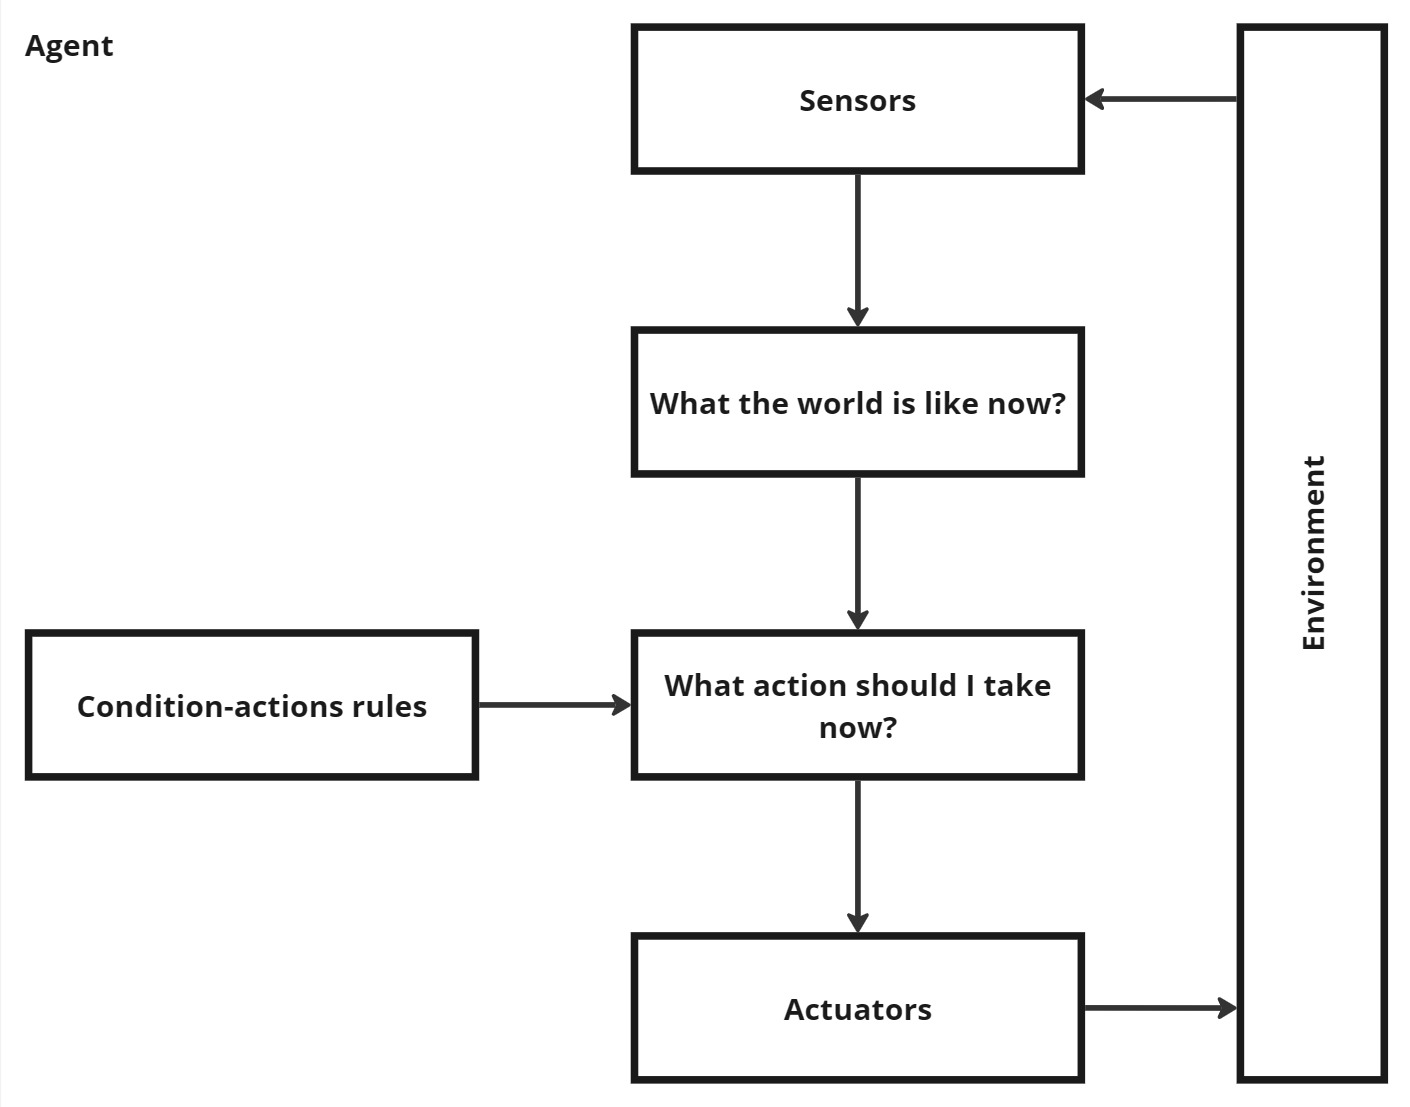
\includegraphics[width=0.75\linewidth]{images/Simple Reflex Agent.jpg}
    \caption{Simple Reflex Agent}
    \label{fig:simple_reflex_agent}
\end{figure}

Simple reflex agents are incredibly simple, but they are of limited intelligence. The agent will work only if the environment is fully observable and even a little bit of unobservability can cause the agent to fail.

Additionally, this kind of agents can fall into infinite loops of actions that are useless, given that have limited intelligence. To avoid this situation, some agents randomize actions, outperforming a deterministic version of the same agent. 

\subsubsection{Model-Based Reflex Agents}
The most effective way to handle partial observability is for the agent to keep track of the part of the world it cannot see at the moment. The agent should maintain some sort of internal state that depends on the percept history and therefore reflects some of the under-observed aspects of the environment.

\begin{figure}[h]
    \centering
    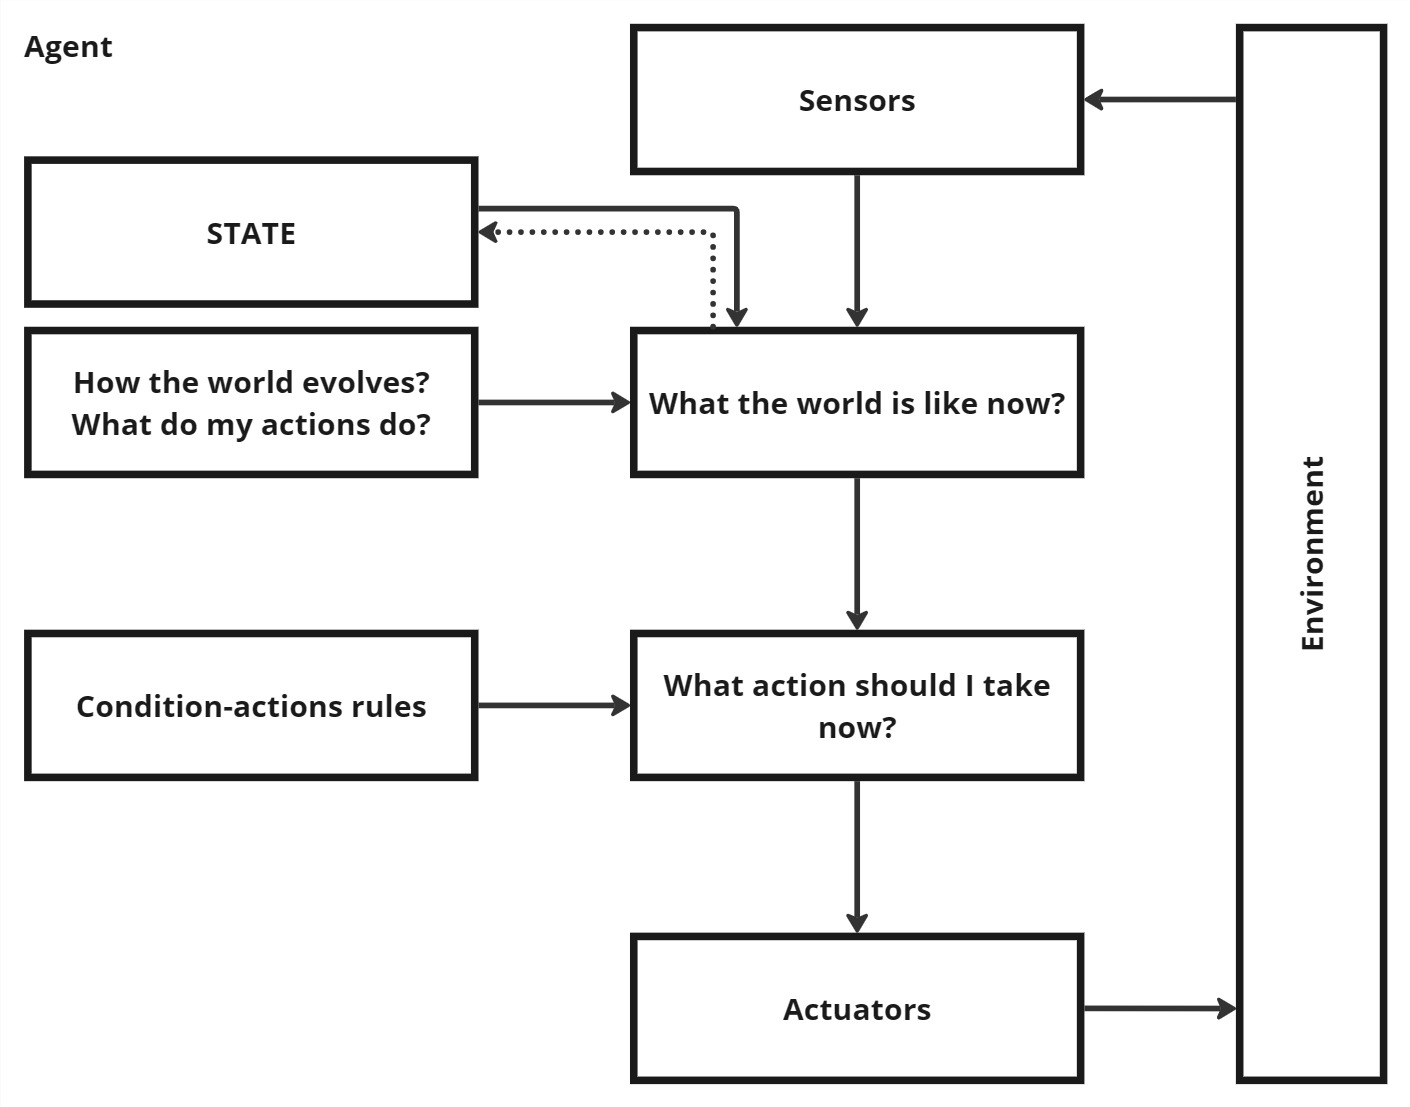
\includegraphics[width=0.75\linewidth]{images/Model Based Reflex Agent.jpg}
    \caption{Model Based Reflex Agent}
    \label{fig:model_based_reflex_agent}
\end{figure}

In order to update this internal state information, two kinds of knowledge are required to be encoded to the agent's program:

\begin{enumerate}
    \item Information about how the world changes over time, which can be divided in two parts:
    \begin{itemize}
        \item The effects of the agent's actions;
        \item How the world evolves independently of the agent.
    \end{itemize}
    This knowledge about how the world evolves is called a \textbf{transition model};
    \item Information about how the state of the world is reflected in the agent's percepts. This kind of knowledge is called \textbf{sensor model}.
\end{enumerate}

Together, the transition model and the sensor model allow the agent to keep track of the state of the world. An agent that uses such models is called a model-based agent.

\subsubsection{Goal-Based Agents}
Knowing something about the current state of the environment is not always enough to decide what to do. As well as the current state description, the agent needs some sort of \textbf{goal}, which are pieces of information that describe desirable situations.

The decision making part of this type of agent is different from the condition-action rules found in the model based reflex agents, in that involves some considerations of the future.

\begin{figure}[h]
    \centering
    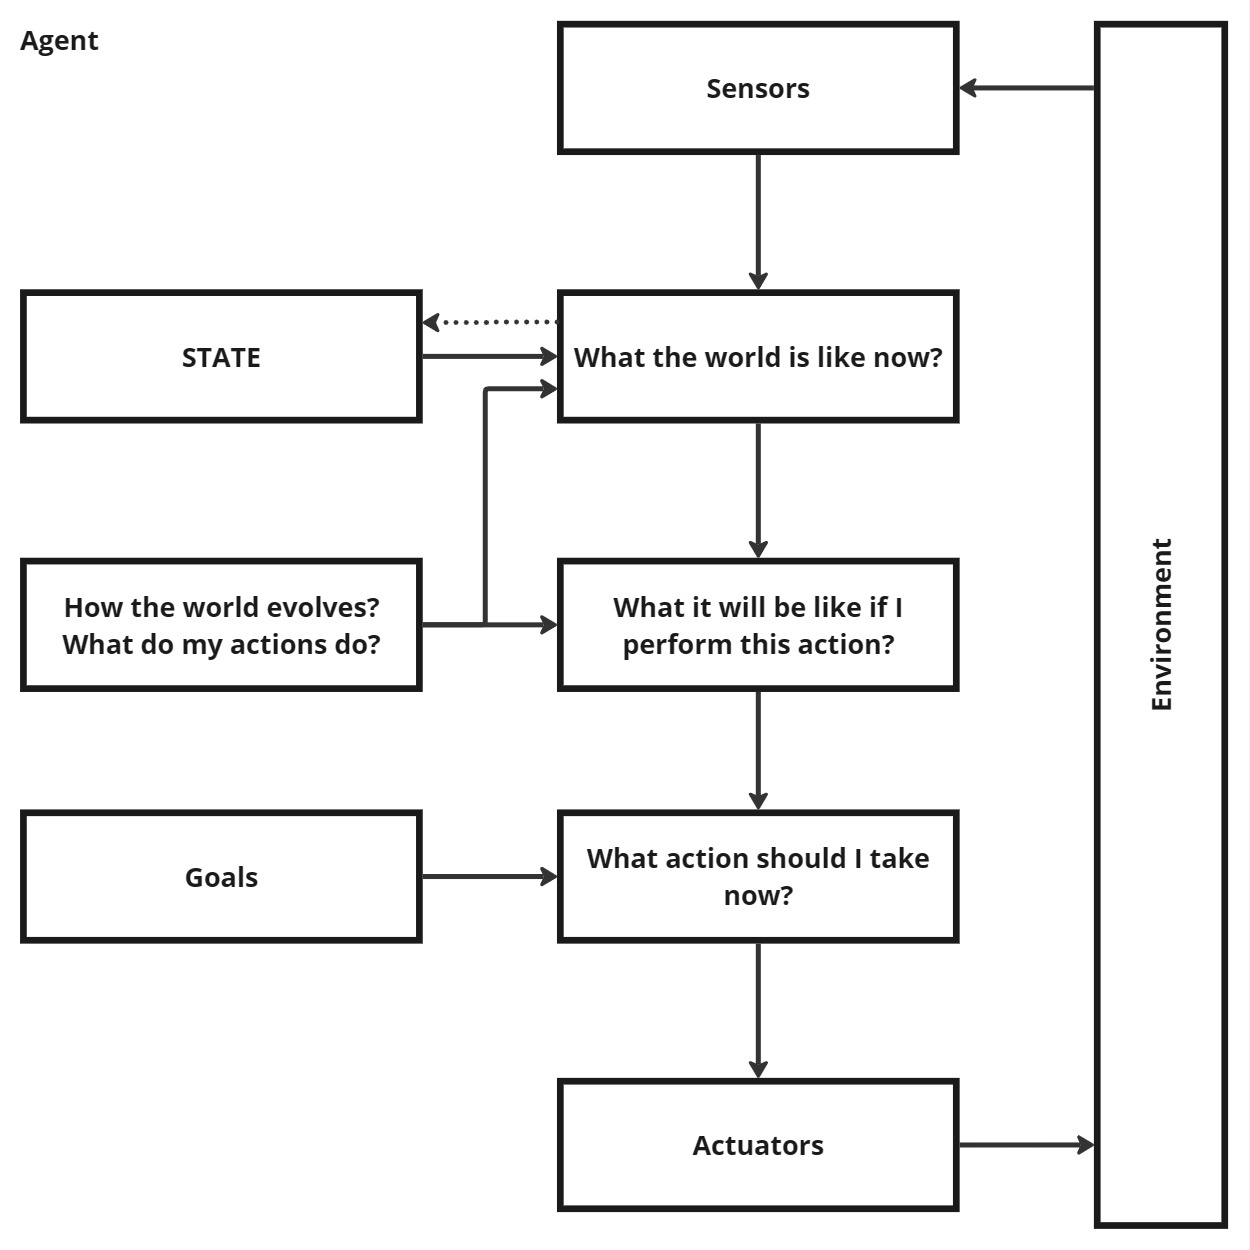
\includegraphics[width=0.75\linewidth]{images/Goal Based Agent.jpg}
    \caption{Goal Based Agent}
    \label{fig:goal_based_agent}
\end{figure}

Agents of this kind may appear less efficient than the ones analyzed up to now, but in reality they are more flexible because the knowledge that supports its decisions is represented explicitly and can be modified, simply by specifying the new goal.

\subsubsection{Utility-Based Agents}
Goals alone are not enough to produce high quality behaviour in most environments, because they only provide a crude distinction between \textit{"happy"} and \textit{"unhappy"} states. A more general performance measure should allow a comparison between different world states according to exactly how happy they would make the agent. In this field, a synonym of happy is \textbf{utility}.  

An agent's utility function is an internalization of the performance measure. Provided that the internal utility function and the external performance measure are in agreement, an agent that chooses actions to maximize its utility function will be rational according to the external performance measure. 

\begin{figure}[h]
    \centering
    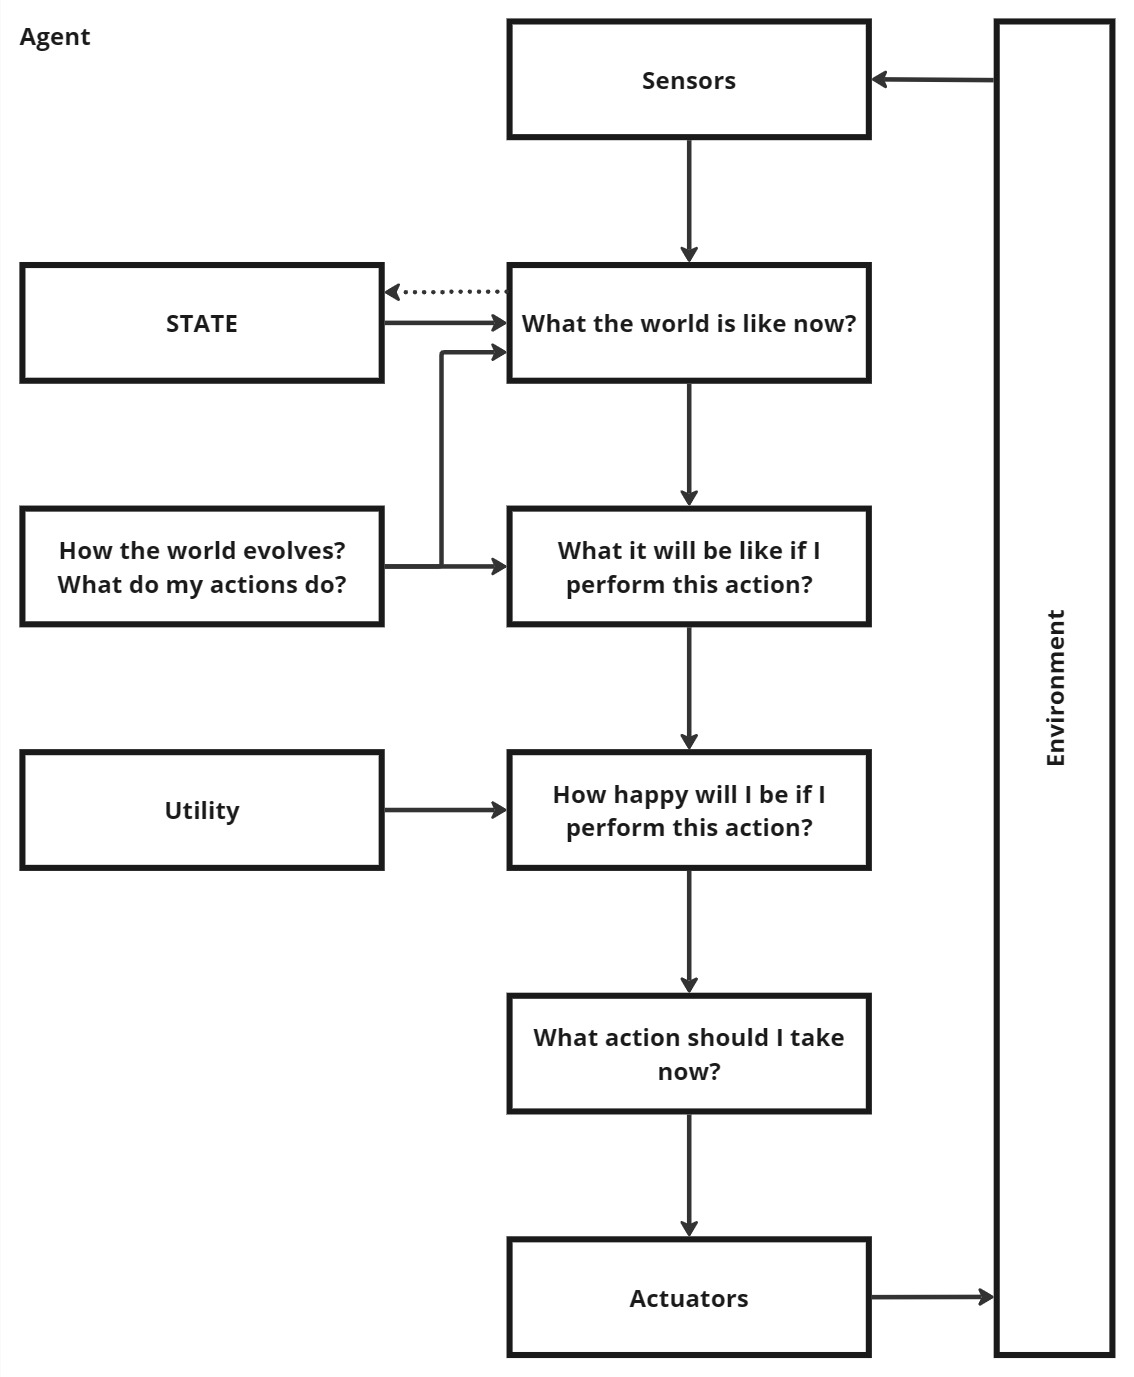
\includegraphics[width=0.75\linewidth]{images/Utility Based Agent.jpg}
    \caption{Utility Based Agent}
    \label{fig:utility_based_agent}
\end{figure}

There are two cases where goals are inadequate, but utility-based agents can still make rational decisions:
\begin{enumerate}
    \item Where there are conflicting goals but only some of them can be achieved: in this case the utility function specifies the right trade-off between the two goals.
    \item Where there are several goals that the agent can aim for, none of which can be achieved with certainty: in this case the utility function provides a way in which the likelihood of success can be weighted against the importance of the goal.
\end{enumerate}

\newpage
\section{Solving Problems by Searching}
We will consider the simplest of environments only: episodic, single agent, fully observable, static, deterministic, discrete and known.

\subsection{Problem Solving Agents}
Any problem solving agent follows a process divided in four phases:
\begin{enumerate}
    \item \textbf{Goal formulation}: the agent adopts the goals. The goal is useful to organize behaviour by limiting the objectives and hence the actions to be considered.
    \item \textbf{Problem formulation}: the agent devises a description of the states and actions necessary to reach the goal. This description is an abstract model of the relevant parts of the world.
    \item \textbf{Search}: before taking any action, the agent simulates sequences of actions in its model, searching until it finds a sequence that reaches the goal. Such a sequence of actions is called a \textbf{solution}. The agent may simulate multiple sequences that do not reach the goal, but eventually it will find a solution, or it will find that no solution is possible.
    \item \textbf{Execution}: the agent executes the actions found in the solution sequence.
\end{enumerate}
\
A search problem can be defined as follows:
\begin{enumerate}
    \item A set of states in which the environment can be in, called the \textbf{state space};
    \item The initial state the agent starts in;
    \item A set of one or more goal states;
    \item The actions available to the agent. Given a state \textit{s}, the function \lstinline{ACTION(s)} return a finite set of actions the agent can perform in the given state. Such state are called \textbf{applicable} in \textit{s};
    \item A transition model, which describes what each action does. The function \lstinline{RESULT(s, a)} returns the state in which the agent will transition to performing action \textit{a} from state \textit{s};
    \item An action cost function, denoted by the \lstinline{ACTION-COST(s, a, s')} function, which returns the numeric cost of performing action \textit{a} in state \textit{s} to reach state \textit{s'}. A problem solving agent should use a cost function that reflects its own performance measure.
\end{enumerate}
\
A sequence of actions is called \textbf{path}. A solution is a path that leads form the initial state to a goal state. The total cost of a path is the sum of the individual costs of every action in the path. An optimal solution is the one that has the lowest path cost among all solutions.

The state space can be represented as a graph in which the vertices are the states and the directed edges between them are the actions the agent can perform. 

The formulation of the problem is the model, an abstract mathematical description. The process of removing irrelevant details from a representation is called \textbf{abstraction}. The abstraction is valid if we can elaborate any abstract solution into a solution in the more detailed world, and is useful if carrying out each of the actions in the solution is easier than the original problem. A good abstraction involves removing as much details as possible while retaining validity and ensuring that the abstract actions are easy to carry out.

\subsection{Search Algorithms}
A search algorithm takes a search problem as input and returns a solution. Most of these type of algorithms are based on a \textbf{search tree data structure} superimposed over the state graph, following various path from the initial state trying to find the one that reaches the goal state. Each node in the search tree corresponds to a state in the state space, while the edges of the tree correspond to actions, as seen in the state graph. The root of the tree corresponds to the initial state of the problem. 

The state space describes the possibly infinite set of states in the world and the actions that allow transitions from one state to another. The search tree describes paths between these states, reaching towards the goal. The search tree may have multiple paths to any given state, but each node has a unique path back to the root of the tree. 

The search tree is created by expanding every node considering the available actions for that state. To do so, we can use the \lstinline{RESULT} function to see where those actions lead to, and generating a new node for each of the resulting states. Now, the algorithm must choose which of these child nodes to consider in order to further expand the tree. This is the core of different search algorithms: they differ from each other for the way they choose the next child to expand in the tree. The set of states that haven't yet been expanded is called \textbf{frontier}, which separates the state space graph from into two regions:
\begin{itemize}
    \item The region of states that have been analyzed and, thus, expanded;
    \item The region of states that haven't yet been expanded.
\end{itemize}

\subsubsection{Best-First Search}
A general approach for deciding which node to expand from the frontier is the \lstinline{BEST-FIRST-SEARCH}, in which we choose a node \textit{n} with minimum value of some evaluation function $f(n)$. On each iteration we choose a node of the frontier with the minimum value of $f(n)$, return it if its state is the goal state, or call the \lstinline{EXPAND} function to generate its child nodes. Each child node is added to the frontier if it has not been reached before, or is re-added if it is reached by a path with a lower costing path. The algorithm returns either an indication of failure if a path is not found, or a node that represents a path to a goal. By using different $f(n)$ functions, we obtain different search algorithms.

\subsubsection{Search Data Structures}
A node in the search tree is represented by a data structure that requires four components:
\begin{enumerate}
    \item \lstinline{node.STATE}: the state to which the node corresponds;
    \item \lstinline{node.PARENT}: the node in the tree that generated this node;
    \item \lstinline{node.ACTION}: the action applied to the parent node's state to generate this node;
    \item \lstinline{node.PATH-COST}: the total cost of the path from the initial state to this node.
\end{enumerate}

Following the \lstinline{PARENT} pointers back from a node, allows to recover the states and actions along the path to that node. Doing so from a goal node to the root of the tree we obtain the solution to the problem we are analyzing. 

Also a data structure to store the frontier is needed. Different data structures make up different types of searching algorithms. The main ones are:
\begin{itemize}
    \item Priority queue: pops the node with the minimum cost according to some evaluation function;
    \item Queue: pops the first node added to the queue;
    \item Stack: pops the last node added to the stack.
\end{itemize}

The reached states can be stored in a hash table, where each key is a state and each value is a node.

\subsubsection{Redundant Paths}
In the search tree might be repeated states, generated by a cycle (called a loopy path) in the graph over which the tree data structure was superimposed. So, there may be cases where the state space ha a finite amount of states, but the complete search tree is infinite, because there are no limits on how many times a path can be traversed in a loop. This kind of paths are called \textbf{redundant paths}, which represent an obstacle in solving the AI related problems. 

If we can eliminate redundant paths, we can make the searching algorithm order of magnitude faster. There are three main approaches to this issue:
\begin{enumerate}
    \item We can store all the previous traversed states in a separate data structure and detect redundant paths in order to keep only the best paths for each state. This approach is appropriate for state spaces where there are many redundant paths and the table of reached states fits in memory.
    \item We can not worry about repeating paths: in some problems is rare or even impossible for two paths to reach the same state, so we can save memory by not tracking reached states and redundant paths. We call a search algorithm a \textbf{graph search} if it checks for redundant paths and \textbf{tree-like search} if it does not.
    \item We can compromise and check only for cycles, but not for redundant paths in general. Since each node has a pointer to its parent node, we can check for cycles simply by following the chain of parents and verify if we land on the same state twice.
\end{enumerate}

\subsubsection{Performance}
An algorithm's performance can be evaluated in four main ways:
\begin{enumerate}
    \item Completeness: whether or not the algorithm is guaranteed to find a solution when there is one and to correctly report failure when there are no solutions;
    \item Cost optimally: whether or not the algorithm finds the most optimal solution, thus the path with the lowest cost of all solutions;
    \item Time and Space complexity: how long does the algorithm take to find a solution and how much memory does it need.
\end{enumerate}

To be complete, a search algorithm must also be \textbf{systematic} in the way it explores an infinite state space, making sure it can eventually reach a goal state which is connected to the initial state. In theoretical computer science, the complexity of a search algorithm is calculated based on the size of the state space graph, which is $|V|+|E|$, where $|V|$ is the number of vertices (or states) of the graph and $|E|$ is the number of edges (or distinct state-action pairs). 

This calculation can be appropriate when the state graph is represented by an explicit data structure, but in AI related problems, this is not always the case. In fact, the graph is generally represented only implicitly by the initial state, actions and transition model. In this case, the complexity of a search algorithm can be measured in terms of the following parameters:
\begin{itemize}
    \item \textit{d} - depth: the number of actions in an optimal solution;
    \item \textit{m}: the maximum number of actions in any path;
    \item \textit{b} - branching factor: the number of successors of a node that need to be considered. 
\end{itemize}

When the branching factor is high, the number of nodes grows quickly and so does the problem complexity. When the depth is large, the closest solution requires more exploration of the search tree, making the algorithm slower. Sometimes, the depth is fixed for any solution.

\subsection{Uninformed Search Strategies}
In uninformed search algorithms no clue is given about how close a state is to the goal and only the information contained in the formulation of the problem itself is used.

\subsubsection{Breadth-First Search}
When all actions inside the state space have the same cost, an appropriate strategy would be a \textbf{breadth-first search}, in which the root node is expanded, then all its successors are expanded next, then their successors and so on. This algorithm is systematic and is therefore complete even on infinite states spaces.

We can implement this strategy by repeatedly calling the \lstinline{BEST-FIRST-SEARCH} algorithm where the evaluation function $f(n)$ is the depth of the node. However, a more efficient implementation would be with a FIFO queue, giving us the correct order of nodes: new nodes (which are deeper than their parents) go to the back of the queue, and old nodes get expanded first, as they are shallower than the new nodes.

Breadth first search always finds a solution with the minimal number of actions, because when it is generating nodes at depth \textit{d}, it has already generated all the nodes at depth \textit{d}-1: if one of them were a solution, it would have been found and the algorithm would have terminated. This means that it is cost optimal for problems where all the actions have the same cost.

In order to calculate time and space complexity, we imagine that all nodes in the tree have \textit{b} successors. In this case, the root of the tree generates \textit{b} nodes, each of which generates \textit{b} more nodes, obtaining $b^2$ nodes for the second level. Each of these generates \textit{b} more nodes, yielding $b^3$ nodes at the third level and so on. All these generated nodes remain in memory, so both time and space complexity are $O(b^d)$.

\subsubsection{Uniform-Cost Search}
When actions in the state space have different costs, an obvious choice would be to apply the \lstinline{BEST-FIRST-SEARCH} algorithm, where the evaluation function is the cost of the path from the root to the current node. This type of search is called \textbf{uniform cost search}. The idea behind this type of algorithm is to expand the nodes in waves of uniform path-cost, instead of uniform depth as in the breadth-first search.

The complexity of this algorithm is characterized in terms of $C^*$, which is the cost of the optimal solution, and $\varepsilon > 0$, which is a lower bound on the cost of each action. Then the algorithm's worst case time and space complexity is $O(b^{1+\lfloor C^*/\varepsilon \rfloor})$, which can be much grater than the $O(b^d)$ found for the breadth-first search algorithm. This is because uniform-cost search can explore very large trees of low-cost actions, before analyzing high-cost and perhaps useful actions.

\subsubsection{Depth-First Search}
This algorithm always expands the deepest node in the frontier list. The search proceeds immediately to the deepest level of the search tree, where the nodes have no successor. Then, if the goal state is not reached, it "backs up" to the next deepest node that still has unexpanded successors. 

It can be implemented using the \lstinline{BEST-FIRST-SEARCH} algorithm, where the evaluation function is the negative of the depth of the node. Alternatively can be implemented using a LIFO queue (also called stack) to represent the frontier: the generated successor nodes are inserted at the front of the frontier and the most recently generated nodes are selected first.

The depth-first search algorithm is not cost-optimal, as it returns the first solution it finds, even if it is not the cheapest one. For finite state spaces, it is efficient and complete, but in cyclic state spaces it can get stuck in an infinite loop. For this reason, some implementations of this algorithm check for loops for each new node in the frontier. Finally, for infinite spaces, it is not systematic either, because it can get stuck in infinite path that are not cycles.

Although it has some harsh downfalls, the depth-first search is generally used for its very limited memory usage: this algorithm has much smaller needs for memory, as it doesn't keep track of the reached states at all and it has a small frontier to save in memory. In fact, the depth-first search algorithm has a time complexity of only $O(b\cdot m)$, where \textit{b} is the branching factor and \textit{m} is the maximum depth of the tree.

\subsubsection{Depth-Limited Search \& Iterative Deepening Search}
We can prevent the depth-first search algorithm to go on endless paths by limiting the depth at which the algorithm can go. We call this algorithm \textbf{depth-limited search}, with limit $\ell$: we treat all nodes at that depth as if they had no successor. The time complexity of this algorithm is $O(b^\ell)$ and the space complexity is $O(b\cdot \ell)$. Unfortunately, if we choose an inappropriate value of $\ell$, the algorithm will fail to reach a solution and it becomes incomplete again. Sometimes a good depth limit can be chosen based on the problem we are trying to solve, but for most problems we will not know a good depth value until we solve the problem.

\textbf{Iterative deepening search} solves the problem of finding a good value for $\ell$ by trying all values until a solution is found or no solutions were found. This approach combines benefits from the depth-first search and breadth-first search algorithms. In fact, like depth-first search, the memory required is modest, spanning from $O(b\cdot d)$ when there is a solution, to $O(b\cdot m)$ on finite state spaces with no solutions. Like breadth-first search, iterative deepening search is optimal for problems where all the actions have the same cost, and is complete on finite acyclic state spaces, or on any finite state space when we check nodes for cycles all the way up the path. The time complexity is $O(b^d)$ when there is a solution, or $O(b^m)$ when there is none.

\subsubsection{Bidirectional Search}
One last strategy we can apply for uninformed search can be to go backward, from the solution to the initial state if the problem is easily reversible. A more efficient way is to combine the two directions into a bidirectional search: this type of search performs two searches in parallel, one \textit{forward} search from the initial state to the goal state, one \textit{backwards} search from a goal state to the initial state.

\subsubsection{Summary}

\begin{table}[h]
    \begin{tabular}{lcccc}
        \multicolumn{1}{l}{} & \multicolumn{2}{c}{\textit{With repeated states}} & \multicolumn{2}{c}{\textit{Without repeated states}} \\
        \multicolumn{1}{r||}{Search Strategy} & \multicolumn{1}{c|}{Complete} & \multicolumn{1}{c|}{Optimal} & \multicolumn{1}{c|}{Complete} & Optimal \\ \hline \hline
        \multicolumn{1}{l||}{\textbf{Breadth-First Search}} & \multicolumn{1}{c|}{YES} & \multicolumn{1}{c|}{YES} & \multicolumn{1}{c|}{YES} & YES \\ \hline
        \multicolumn{1}{l||}{\textbf{Uniform-Cost Search}} & \multicolumn{1}{c|}{YES} & \multicolumn{1}{c|}{YES} & \multicolumn{1}{c|}{YES} & YES \\ \hline
        \multicolumn{1}{l||}{\textbf{Depth-First Search}} & \multicolumn{1}{c|}{NO} & \multicolumn{1}{c|}{NO} & \multicolumn{1}{c|}{YES} & NO \\ \hline
        \multicolumn{1}{l||}{\textbf{Limited-Depth Search}} & \multicolumn{1}{c|}{NO} & \multicolumn{1}{c|}{NO} & \multicolumn{1}{c|}{NO} & NO \\ \hline
        \multicolumn{1}{l||}{\textbf{Iterative Deepening}} & \multicolumn{1}{c|}{YES} & \multicolumn{1}{c|}{YES} & \multicolumn{1}{c|}{YES} & YES
    \end{tabular}
    \caption{Strategy comparison}
    \label{tab:strategy_comparison}
\end{table}

\begin{table}[h]
    \centering
    \begin{tabular}{l||c|c}
        Strategy & S(n) & T(n) \\ \hline \hline
        \textbf{Breadth-First Search} & $O(b^d)$  & $O(b^{d+1})$ \\ \hline
        \textbf{Uniform-Cost Search} & $O(b^{1+\lfloor C^*/\varepsilon \rfloor})$ & $O(b^{1+\lfloor C^*/\varepsilon \rfloor})$ \\ \hline
        \textbf{Depth-First Search} & $O(bm)$ & $O(b^m)$ \\ \hline
        \textbf{Limited-Depth Search} & $O(b\ell)$ & $O(b^\ell)$ \\ \hline
        \textbf{Iterative Deepening} & $O(bd)$ & $O(b^d)$ \\
    \end{tabular}
    \caption{Strategy Complexity}
    \label{tab:strategy_complexity}
\end{table}

Where:
\begin{itemize}
    \item $b$ is the number of successors of a node that need to be considered;
    \item $d$ is the number of actions in an optimal solution;
    \item $m$ is the maximum number of actions in any path;
    \item $C^*$ is the cost of the optimal solution;
    \item $\varepsilon$ is the lower bound on the cost of each action;
    \item $\ell$ is the depth limit;
\end{itemize}

\subsection{Informed Search Strategies}
In informed search algorithms, specific knowledge that is not contained in the problem formulation is exploited to solve the problem itself. This strategy selects a node from the frontier according to an evaluation function $f(n)$, which provides an estimate of how much a node is "promising". There are two main ways to calculate the evaluation function:
\begin{enumerate}
    \item Greedy best-first search;
    \item A* search.
\end{enumerate}

Conventionally, the most promising nodes have a small value of the evaluation function $f(n)$, so the frontier is implemented as a priority queue ordered in increasing order of $f(n)$. Thus, nodes with the minimum $f(n)$ are chosen first.

\subsubsection{Greedy Best-First Search}
Greedy best-first search algorithms use an evaluation function that is equal to the \textbf{heuristic function} $h(n)$, which gives the \textit{estimated} cost of the cheapest path from the state at node $n$ to a goal state. To apply the greedy best-first search, the function $h(n)$ must be known. Note that, the heuristic is an estimate, not an actual cost: if we knew the actual cost of the path, the problem would have already been solved.

There are many heuristic functions we can choose for every given problem, but there are some more accurate than others. In fact, given two heuristic functions $h_1(n)$ and $h_2(n)$, such that $h_1(n)\le h_2(n)$ for any node $n$, $h_2$ is said to dominate $h_1$ since each node expanded using $h_2$ is also expanded using $h_1$. In this case we say that the function $h_2$ is more accurate, or more informed, than the function $h_1$.

Greedy best-first search is neither complete nor optimal, as it can get stuck in an infinite loop. The time and space complexity of this algorithm in the worst-case scenario are both $O(b^m)$, where $m$ is the maximum depth of the search tree (which could be infinite).

\subsubsection{A* Search}
The most used informed search algorithm is \textbf{A* search}, a best-first search that uses the evaluation function $f(n) = g(n) + h(n)$, where:
\begin{itemize}
    \item $g(n)$ is the path cost from the initial state to node $n$ (what we know for sure);
    \item $h(n)$ is the estimate cost of the shortest path from $n$ to a goal state (what we are estimating).
\end{itemize}
Put in simpler words, $f(n)$ is the estimated cost of the best path that continue from the state $n$ to a goal state. By using both the cost so far and the estimated cost of reaching the goal, A* can lead the agent away from suboptimal paths.

A* search is complete and optimal for tree-search when the function $h(n)$ is \textbf{admissible}. A heuristic function is admissible when, for each node $n$, it is true that 
    \[0 \le h(n) \le h^*(n)\]
where $h^*(n)$ represents the actual cost from the given node to a solution node. When $n$ is a goal state, $h(n)$ should be zero. An admissible heuristic is \textit{"optimistic"} since it always underestimates the true cost to reach the goal. In fact an it can be seen as the cost of an optimal solution to a relaxed problem, obtained by removing the constraints.

A* search is also complete and optimal for graph-search when the function $h(n)$ is \textbf{consistent}. An heuristic function is consistent when, for every node $n$ and every successor $n'$ generated from $n$ by action $a$, it is true that 
\[h(n)\le c(n,a,n') + h(n') \;\; \textnormal{(triangular inequality)}\]
When $n$ is a goal state, $h(n)$ should be zero. Every consistent heuristic function is also an admissible one, but not vice versa. Consistency is a stronger property than admissibility, because graph-search is more constrained since it does not consider nodes corresponding to the same state, thus it requires a stronger property to guarantee completeness and optimality. In addition, with a consistent heuristic, the first time we reach a state it will be on an optimal path, so we never have to re-add a state to the frontier and never have to change an entry in the \textit{reached} set.

There are many types of consistent heuristic functions, but some of them are uninteresting: for example, the heuristic function $h_0(n) = 0 \;\; \forall n$ is consistent and admissible, but it implements a uniform-cost search (uninformed search algorithm), so it is not really that interesting.

A special variation of the A* search is the \textbf{weighted A* algorithm}. It introduces a weight factor $w$, which is $1 \le w < \infty$, over the heuristic functions so that $f(n) = g(n) + w \cdot h(n)$. The theoretical properties of the simple A* search do not apply anymore, but this extension of the algorithm can be more efficient and solve search problems quicker.

The last, and most successful, variation of A* search is the \textbf{iterative-deepening A* search} (IDA* search), which reduces memory requirements by applying a limit to the values of the evaluation function $f(n)$. It is to A* what iterative-deepening was to depth-first search: IDA* gives all the benefits of A* without the requirement to keep the reached states in memory, at the cost of visiting some states multiple times. In IDA* the cutoff value is the $f-cost (g+h)$; at each iteration, the cutoff value is the smallest $f-cost$ of any node that exceeded the cutoff on the previous iteration. IDA* search is complete and optimal when the heuristic function $h(n)$ is admissible.

\newpage
\section{Constraint Satisfaction Problems}
In standard search, the basic idea is that problems can be solved by searching the state space, that is a graph in which nodes represent states and edges between them represent actions. In this type of search algorithms, the states are atomic, indivisible, like a \textit{black box}: for each problem, we need domain-specific heuristic function to describe the transition between states.

In \textbf{constraint satisfaction problems}, \textbf{CSP} for short, we break open this black box by using a factored representation for each state, that consists of a set of variables, each of which have a value. A CSP is solved if each variable has a value that satisfies all the constraints on that variable.

CSP search algorithms take advantage of the structure of states and use a general heuristic to enable the solution of complex problems. The main idea is that we can eliminate large portions of the search space by identifying values that violate constraints on variables.  \\

\begin{definition}
A CSP consists of three components:
\begin{itemize}
    \item $\mathcal{X} =\{X_1, ..., X_n\}$ is a set of variables;
    \item $\mathcal{D} =\{D_1, ..., D_n\}$ is a set of domains, one for each variable;
    \item $\mathcal{C}$ is a set of constraints that specify valid combinations of values.
\end{itemize}
\end{definition}

A domain $D_i$ is a set of allowable values $\{v_1, ..., v_k\}$ for each variable $X_i$. Each constraint $\mathcal{C}_j$ consists of a pair $<scope,\; rel>$, where $scope$ is a tuple of variables that participate in the constraint, and $rel$ is a relation that defines the valid values for those variables. A relation can be represented as am explicit set of all tuples of values that satisfy the constraint, or as a function that can compute whether or not a tuple is a member of the solution.

The goal of the CSP is to assign values to the variables, such that 
\[\{X_i=v_i, X_j=v_j, ...\}.\] 
An assignment is \textbf{consistent} if does not violate any constraints and is \textbf{complete} if all variables are assigned a value. A solution to a CSP is a consistent and complete assignment. If all the domains have fixed size $d$, there are $O(d^n)$ complete assignments possible.

Every CSP can be visualized as a constraint graph: the nodes of the graph correspond to variables of the problem and the edge connects any two variables that participate in a constraint. This type of representation for the problem can dramatically speed up the search problem. Additionally, we will consider only binary constraints, in which only two variables are involved, because higher order constraints can be transformed in a CSP with only binary constraints through simple transformations.

\subsection{Constraints Propagation - Arc consistency}
A variable in a CSP problem is arc-consistent if every value in its domain satisfies the variable's binary constraints. More formally, $X_i$ is arc-consistent with respect to another variable $X_j$ if there is some value in the domain $D_j$ that satisfies the binary constraint in the arch $(X_i, X_j)$.

The most popular algorithm for enforcing the arc-consistency property on a CSP problem is called \textbf{AC-3}, which maintains a queue of arcs to consider. Initially, the queue contains all the arcs in the CSP. Then, the algorithm pops off an arbitrary arc $(X_i, X_j)$ and makes $X_i$ arc-consistent with respect to $X_j$. If this leaves $D_i$ unchanged, the algorithm moves on the next arc, but if this operation revises the domain $D_i$ (making it smaller), then we add to the queue all arcs $X_k, X_i$, where $X_k$ is a neighbor of $X_i$. This is necessary because, by reducing $D_i$, we might enable further reductions in $D_k$, even if we've already applied the algorithm to that node. If $D_i$ is revised down to nothing, then we know that the whole CSP problem has no consistent solution and the algorithm can immediately return failure. Otherwise, we keep checking, trying to remove values from the domains of variables until no more arcs are in the queue. At this point we are left with a CSP equivalent to the initial one, but the arc consistent one will be faster to search because its variables have smaller domains.

The complexity of AC-3 is $O(cd^3)$ in the worst case scenario.

\subsection{Backtracking Search for CSP}
Sometimes we can finish the constraint propagation process and still have variables with multiple possible values. In this case we have to search a solution. For a CSP problem with $n$ variables of domain size $d$ we would end up with a search tree where all the complete assignments are leaf nodes at depth $n$. But, the branching factor at the top level would be $nd$ because any of $d$ values can be assigned to any of $n$ variables. At the next level, the branching factor is $(n-1)d$ and so on for $n$ levels. So the tree has $n!d^n$ leaves, even though there are only $d^n$ possible assignments.

We can remove the $n!$ factor by recognizing that CSP have the \textbf{commutative property}. A problem is said to be commutative if the order of any given set of actions does not matter. In CSPs it makes no difference if we first assign a value to a variable first and then to another, or the other way around. Therefore, we need only consider a single variable at each node in the search tree. At each level of the tree we must choose which variable we will deal with, but we never have to backtrack over that choice. 

Backtracking search algorithm for CSP repeatedly chooses an unassigned variable and tries all values in the domain of that variable in turn, trying to extend each one into a solution recursively. If the call succeeds, the solution is returned, otherwise the assignment is restored to the previous state, from which we try all the remaining values. If no value works we return a failure. This algorithm can be improved by using domain-independent heuristics that take advantage of the factored representation of the CSP.

\subsubsection{Variable ordering}
There are various strategies we can implement in order to select an unassigned variable. The simplest one is to choose variables in order $\{X_1, X_2, ..., X_n\}$ or randomly. Though, there are better heuristics, like choosing the variable with the fewest possible values, called \textbf{minimum-remaining-values} (\textbf{MRV}). This strategy is also called "fail-first" as it picks a variable that is most likely to cause a failure soon, thereby pruning the tree.

Another strategy is the \textbf{degree heuristic}, which attempts to reduce the branching factor on future choices by selecting the variable that is involved in the largest number of constraints on other unassigned variables. The MRV heuristic is usually more powerful, but the degree heuristic can be useful as a tie-breaker.

Once a variable is selected, the algorithm must decide on the order ti examine its values. An efficient algorithm is the \textbf{least-constraining-value} heuristic, which prefers the value that rules out the fewest choices for the neighboring variables in the constraint graph.

We learned that variables should be selected following the "fail-first" principle, while its values should follow the "fail-last" principle. This is because every variable has to be assigned eventually, so by choosing the ones that are likely to fail first, we will have fewer successful assignments to backtrack over. On the other hand, for value ordering we need only one solution, so it makes sense to look for the most likely values first.

\subsubsection{Forward Checking}
The AC-3 algorithm can reduce the domains of variables before we begin the search, but inference can be more powerful during the search. One simple type of inference is \textbf{forward checking}. Whenever a variable $X$ is assigned, the forward checking algorithm establishes arc consistency for it: for each unassigned variable $Y$ connected to $X$ by a constraint, it deletes from $Y$'s domain any value that is consistent with the value chosen for $X$. For many applications, the search is more effective if we combine the MRV algorithm with forward checking. A problem with forward checking is that although it detects many inconsistencies, it does not detect them all.

\subsection{Local Search}
We can efficiently solve CSPs using another paradigm: \textbf{local search}. It uses a complete state formulation where each state assigns a value to every variable, and the search changes the value of one variable at a time. To do so, it uses the \textbf{hill-climbing} algorithm: considering the states of a problem as laid out in a state-space landscape, each point has an "elevation", defined by the value of the objective function; the problems is narrowed down to finding the global maximum value. The only problem in this kind of algorithms is that they can stop at local maxima, yielding a sub-optimal solution.

\newpage
\section{Adversarial Search and Games}
Adversarial search problems are a set of problems in which we explore competitive environments, where two or more agents have conflicting goals.

\subsection{Two-Player Zero-Sum Games}
The most studied problems in AI are the deterministic, two-player, turn-taking, perfect information (fully observable) and zero-sum (there's always one winning player) games. In game theory the terms move and position are used as synonim for action and state respectively.

The analyzed games will always have two involved players, called MAX and MIN, in which MAX moves first and then the players take turns moving until the game is over. 

A game can formally be defined with the following elements:
\begin{itemize}
    \item $S_0$: the initial state, which specifies how the game is set up at the start;
    \item \lstinline{To-Move(s)}: the player whose turn it is to move in state $s$;
    \item \lstinline{Actions(s)}: the set of legal moves the player can do in state $s$;
    \item \lstinline{Result(s, a)}: the transition model, which defines the state resulting from the taking action $a$ in state $s$;
    \item \lstinline{Is-Terminal(s)}: the terminal test, which returns true if the game is in a terminal state, false otherwise;
    \item \lstinline{Utility(s, p)}: the utility function, which defines the final numeric value to player $p$ when the game ends in terminal state $s$.    
\end{itemize}

The initial state, the \lstinline{Actions} function and the \lstinline{Result} one define the \textbf{state space graph}, where the vertices represent the states and the edges the moves. As always a \textbf{search tree} can be superimposed on the graph (or on a particular part of it), to determine what moves to make next. We can define the complete \textbf{game tree} as the search tree that follows every possible path all the way down to a terminal state.
Leaf nodes contain the utility value of the terminal state from the point of view of MAX: high values are good for MAX and bad from MIN.

\subsection{Optimal Decisions}
Given a game tree, the optimal strategy can be determined by evaluating the \textbf{minimax} value of each state of the tree, which is indicated with \lstinline{MINIMAX(s)}. This value is the utility for MAX being in that state, \textit{assuming that both players play optimally}. The minimax value of a terminal state is just its utility. In any terminal space, MAX prefers to move to a state of maximum value when it's his turn to move, while MIN prefers a state of minimum, which is minimum value for MAX (thus maximum value for MIN). So the minimax function is calculated as follows:
\begin{multline}
    MINIMAX(s) = \\
    \begin{cases}
        Utility(s, MAX) & if \;\; Is-Terminal(s) \\
        \max_{a\in Actions(s)} MINIMAX(Result(s, a)) & if \;\; To-Move(s) = MAX \\
        \min_{a \in Actions(s)} MINIMAX(Result(s, a)) & if \;\; To-Move(s) = MIN        
    \end{cases}
\end{multline}

This definition of optimal play for MAX assumes that MIN also plays optimally. If MIN does not play optimally, then MAX will be at least as good as against an optimal player, possibly better.

\subsubsection{Minimax search algorithm}
By using the \lstinline{MINIMAX} function, we can build a \textbf{minimax search algorithm} that finds the best move for MAX, by trying all actions and choosing the one whose resulting state has the highest \lstinline{MINIMAX} value. This algorithm is recursive and proceeds all the way down to the leaves of the tree and than backs up the minimax values through the tree as the recursion unwinds.

The algorithm performs a complete depth-first exploration of the game tree: if the maximum depth of the tree is $m$ and there are $b$ legal moves at each point, then the time complexity of the minimax algorithm is $O(b^m)$ and the space complexity is $O(bm)$. The exponential time complexity makes the minimax algorithm impractical for complex games. By approximating the analysis in various ways, we can write more efficient algorithms.

\subsubsection{Alpha-Beta pruning}
As seen in the previous section, the number of game states is exponential in the depth of the tree. We can speed up the algorithms by \textbf{pruning} large portions of the tree that make no difference to the outcome. We will examine the \textbf{alpha-beta pruning} technique.

Sometimes the minimax value is independent from the value of other nodes. Let $n$ be a node of the tree, such that the player has a choice of moving to $n$: if the player has a better option either at the same level as $n$ or higher up, the player will never move to $n$. So, once we have found out enough about $n$ to reach this conclusion, we can prune the entire subtree with root in $n$. 

The alpha-beta pruning gets its name from the two extra parameters passed to the \lstinline{Max-Value(}$state, \alpha, \beta$\lstinline{)} function, that describe bounds on the backed-up values that appear anywhere along the path:
\begin{itemize}
    \item $\alpha$ is the value of the best choice we have found so far at any choice point along the path for MAX. We can think of $\alpha$ as "\textit{at least}".
    \item $\beta$ is the value of the best choice we have found so far at any choice point along the path for MIN. We can think of $\beta$ as "\textit{at most}".
\end{itemize}

Alpha-beta search updates the values of $\alpha$ and $\beta$ as it goes along and prunes the remaining branches at node as soon as the value of the current node is known to be worse than the current $\alpha$ or $\beta$ value for MAX or MIN respectively.

In order to make Alpha-beta pruning highly efficient we need to make some clarifications about the order in which we examine the states. One improvement we can make is to examine first the successors that are likely to be best. If this could be done perfectly, alpha-beta pruning would need to examine only $O(b^{m/2})$ nodes to pick the best move, instead of the $O(b^m)$ required by the minimax algorithm. So alpha-beta pruning with perfect move ordering can solve a tree roughly twice as deep as minimax in the same amount of time.

\subsection{Heuristics for Alpha-Beta Tree Search}
To make efficient use of the limited computational power and time, we can cut off the search early by applying a \textbf{heuristic evaluation function} ti states, effectively treating non-terminal nodes as if they were terminal. To do so, we replace the \lstinline{Utility} function with an \lstinline{Evaluation} function, which determines the state's utility. We also replace the terminal test by a \textbf{cutoff test}, which must return true for the terminal states and must decide when to cut off the search, based on the search depth and other properties.

The \lstinline{Eval(s, p)} function returns an estimate of the expected utility of state $s$ to player $p$, which should be strongly correlated with the actual chances of winning. Most of the evaluation functions work by calculating various \textbf{features} if the state. The features taken together define various categories, called \textit{equivalence classes} of states: the states in each category have the same values for all the features. Any given category will contain some states that lead to winning, some that lead to draws and some others that lead to losses. Most of the evaluation functions compute separate numerical contributions from each feature and then combine them in one total value, using a \textbf{weighted linear function}:
\[Eval(s) = w_1f_1(s)+w_2f_2(s)+\cdots+w_nf_n(s) = \sum_{i=1}^{n}w_if_i(s)\]

\noindent where $f_i$ is a feature of the position and $w_i$ is a weight, saying how important a feature is. This sum should be normalized in order to get a value in the range between 0 and 1.

\subsection{Stochastic Games}
\textbf{Stochastic Games} bring us a little closer to the real world by adding a random element in the computation. In this case, the game tree must include \textbf{chance nodes} (represented in circles) in addition to MAX and MIN nodes. The branches leading from each chance node denote the random probability. 

In this kind of games, we still want to pick the move that leads to the best decision. However, positions do not have definite minmax values. Instead, we can only calculate the \textbf{expected value} of a position: the average overall possible outcome of the chance nodes. This leads to the \textbf{expectiminimax value} for games with chance nodes, a generalization of the minimax value for deterministic games. Terminal, MAX and MIN nodes work exactly the same as before, but for chance nodes we compute the expected value, which is the sum of the value over all outcomes, weighted by the probability of each chance action:

\begin{multline}
    EXPECTIMINIMAX(s) = \\
    \begin{cases}
        Utility(s, MAX) & if \;\; Is-Terminal(s) \\
        \max_{a\in Actions(s)} EXPECTIMINIMAX(Result(s, a)) & if \;\; To-Move(s) = MAX \\
        \min_{a \in Actions(s)} EXPECTIMINIMAX(Result(s, a)) & if \;\; To-Move(s) = MIN \\
        \Sigma_{r}P(r) EXPECTIMINIMAX(Result(s, a)) & if\;\; To-Move(s) = CHANCE\\
    \end{cases}
\end{multline}

Where $r$ represents the chance event and $Result(s, r)$ is the same state as $s$, with the additional fact that the result of the dice roll is $r$

\subsection{Monte Carlo Tree Search}
For games with large state spaces and high branching factor the algorithms used up to now are impractical. Furthermore there are cases in which we don't now the domain very well and the branches are all equally promising. In this cases, the best algorithm to use is the \textbf{Monte Carlo Tree Search}. It does not use a heuristic function to solve the problem, but instead the value of a state is determined as the average utility over a number of simulations of complete games starting from that state. A simulation, also called \textbf{playout} or \textbf{rollout}, chooses moves first for one player, the for the other, repeating until a terminal position is reached. At that point, the rules of the game decide who has won or lost, determining the "win percentage".

In order to get useful information from the playout we need a \textbf{playout policy}, that biases the moves towards good ones instead of randomly choosing between the available ones. Once a policy has been chosen, we need to decide from what position to start the playouts and how many do we need to allocate for each position. The simplest solution is to start from the current state of the game and compute $N$ simulations, tracking down which of the possible moves from the current position has the highest win percentage.

While for stochastic games this converges to optimal play as $N$ increases, for most game it is not sufficient: we need a selection policy that focuses on the important parts of the game tree. It should balance two main factors: \textbf{exploration} of states that have had few playouts, and \textbf{exploitation} of states that have done well in past playouts, to get more accurate estimate of their value.

Monte Carlo Tree Search does that by maintaining a search tree and growing it on each iteration of the following steps:
\begin{enumerate}
    \item \textbf{Selection}: starting at the root of the search tree, we choose a move guided by the selection policy, leading to a successor node, and repeat the process moving down the tree to a leaf;
    \item \textbf{Expansion}: we grow the search tree by generating one or more children of the selected node;
    \item \textbf{Simulation}: we perform a playout from the newly generated child node, choosing moves for both players according to the playout policy;
    \item \textbf{Back-propagation}: we use the result of the simulation to update all the search tree nodes going up to the root.
\end{enumerate}

We repeat these four steps either for a set number of iterations or until the allotted time has expired, and then return the move with the highest number of playouts.

One effective selection policy is the \textbf{upper confidence bounds applied to trees} (\textbf{UCT}), which ranks each possible move based on an upper confidence bound formula called UCB1. For a given node $n$, the formula is:

\[UCB1(n) = \frac{U(n)}{N(n)}+C\cdot\sqrt{\frac{\log{N(Parent(n))}}{N(n)}}\]

\noindent where $U(n)$ is the total utility of all playouts that went through node $n$, $N(n)$ is the number of playouts through node $n$, and $Parent(n)$ is the parent node of $n$ in the tree. Thus, the first term of the equation is the exploitation term, which calculates the average utility of $n$. The second term of the equation, the one with the square root, is the exploration term. We see that in the numerator we have the logarithm of the number of times we have explored the parent of the current node: this means that if we are selecting $n$ some non zero percentage of the time, the exploration term goes to zero as the counts increases, and eventually the playouts are given to the node with the highest average utility. $C$ is a constant that balances exploitation and exploration.

\newpage
\section{Learning Agents}
Any type of agent, such as model-based, goal-based or utility-based, can be built as a learning agent to improve their performance. Learning allows the agent to operate in a initially unknown environment and to become more competent than its initial knowledge alone might allow. 

\begin{figure}[h]
    \centering
    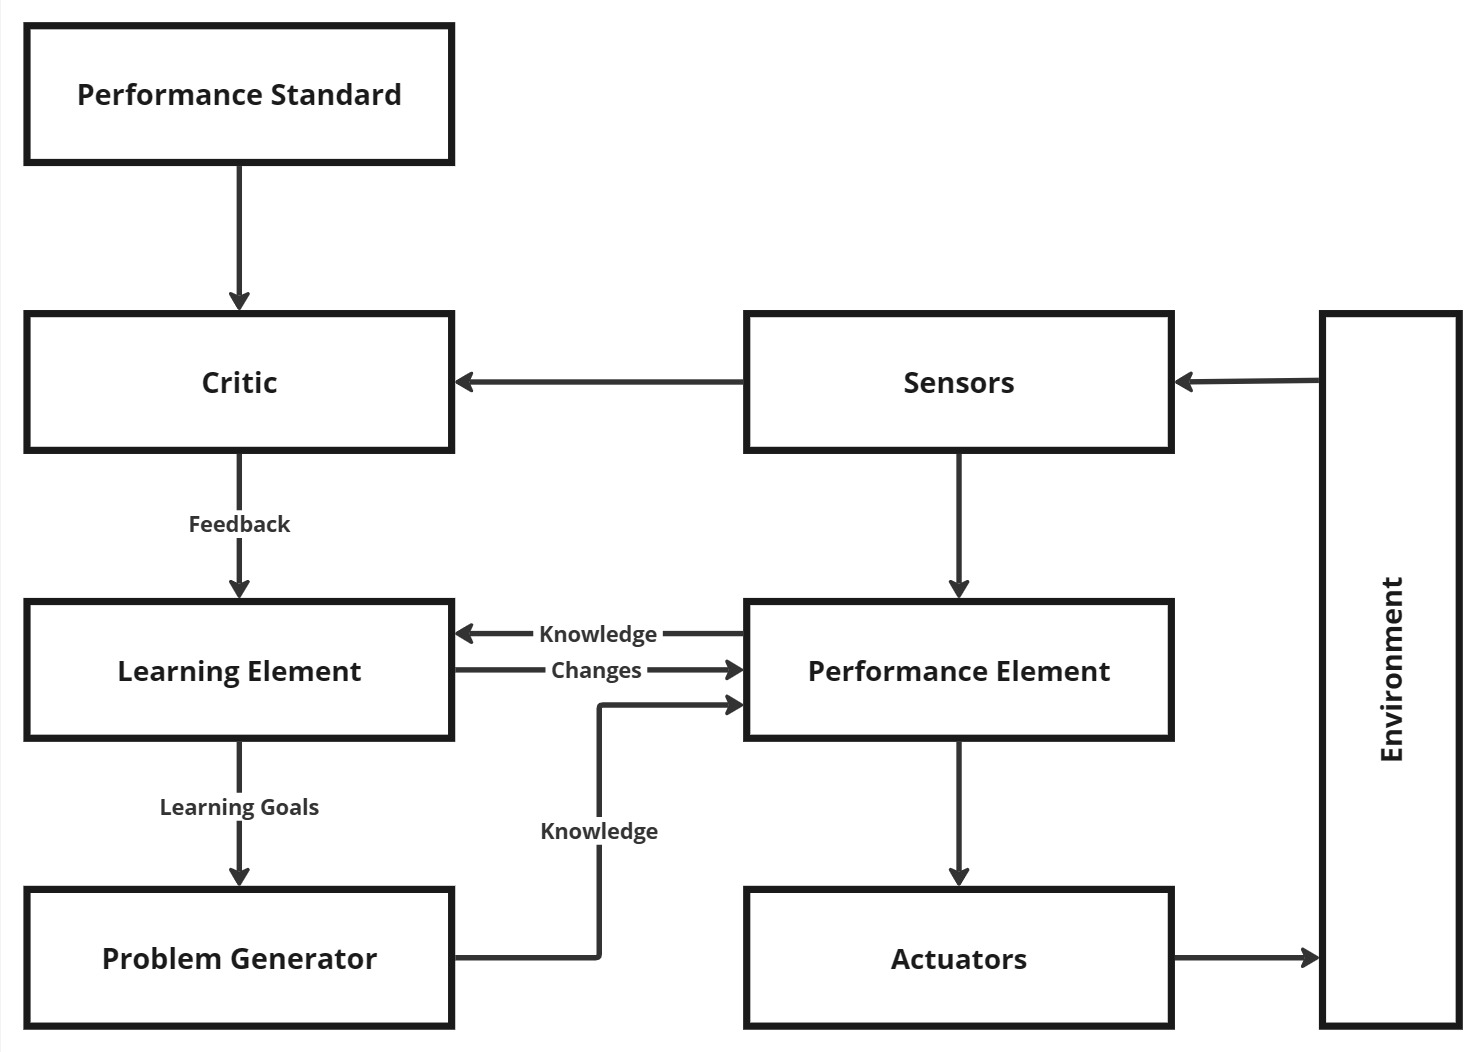
\includegraphics[width=0.75\linewidth]{images/Learning Agent.jpg}
    \caption{Learning Agent}
    \label{fig:learning_agent}
\end{figure}

It can be divided in four conceptual components:
\begin{enumerate}
    \item Learning element: responsible for making improvements;
    \item Performance element: analyzes the sensor input data and selects external actions. It's what we considered as the entire agent in the previous chapter;
    \item Critic: provides feedback on the actions taken by the agent and determines how the performance element should be modified to improve performance;
    \item Problem generator: suggests exploratory actions that lead to new and informative experiences. 
\end{enumerate}
\
\begin{definition}
    A computer program is said to learn from experience \textbf{E} with respect to some class of tasks \textbf{T} and performance measure \textbf{P}, if it improves with the given experience.
\end{definition}

Formally, Machine Learning is a field of AI focused on building algorithms capable of learning by extracting knowledge from experience. The goal is to build programs that can make informed decisions on new unseen data.

\begin{figure}[h]
    \centering
    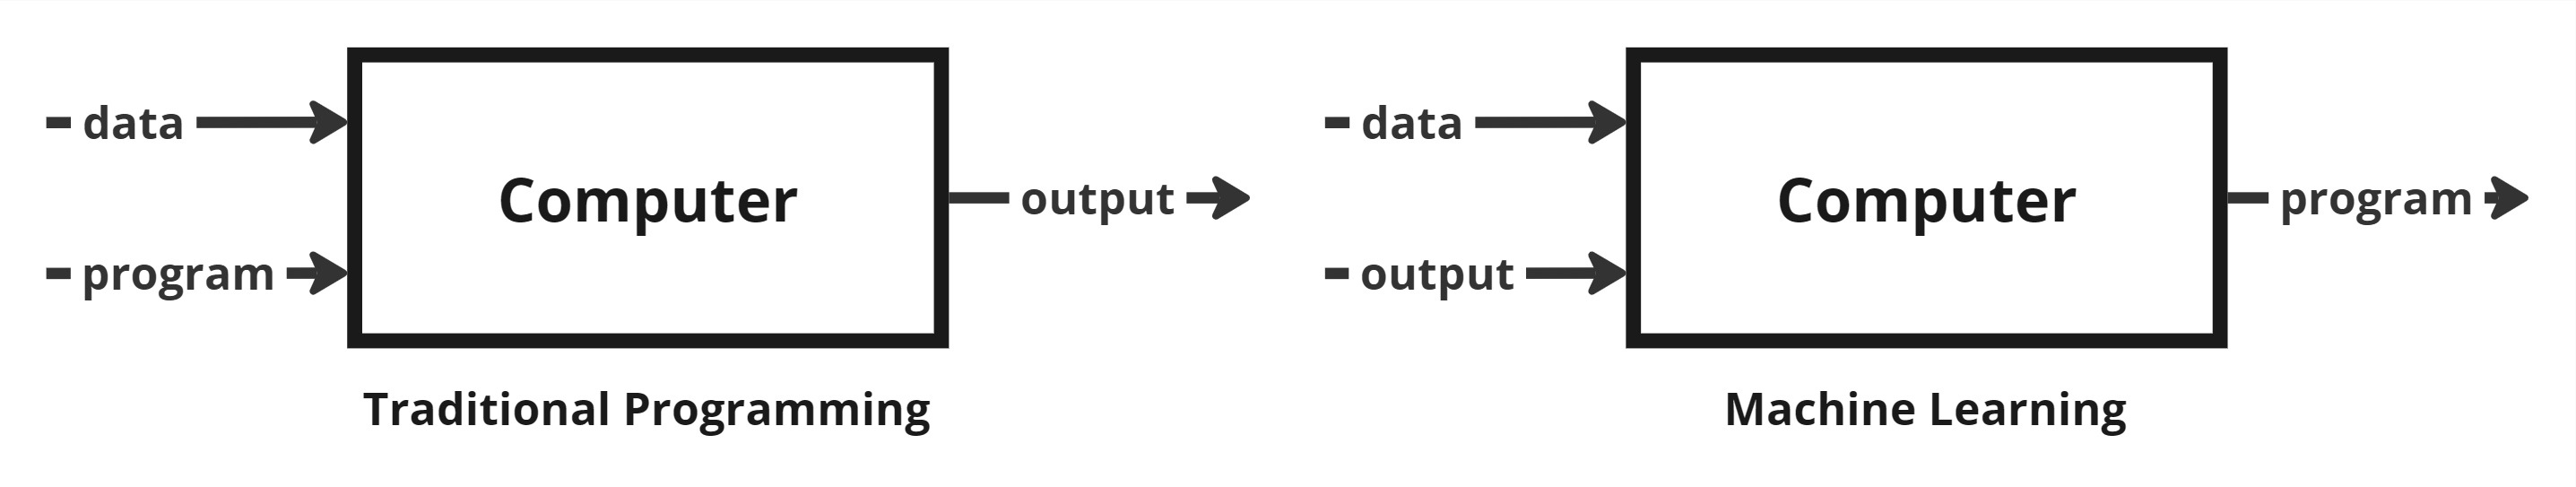
\includegraphics[width=0.75\linewidth]{images/Machine Learning Paradigm.jpg}
    \caption{Machine Learning Paradigm}
    \label{fig:machine_learning_paradigm}
\end{figure}

There are three main types of machine learning agents:
\begin{enumerate}
    \item \textbf{Supervised Learning}: given a set of desired outputs $y_1, ..., y_n$, the agent learns to produce the correct output for a new set of unseen values. The outputs from which the agent learns are called \textbf{labels}.
    \item \textbf{Unsupervised Learning}: the agent exploits patterns and regularities in the experience collected (encoded as a dataset $D = x_1, ..., x_n$). In this case there's no desired output to predict and no feedback. The most common unsupervised learning task is called \textbf{clustering}, which detects useful clusters from the input example.
    \item \textbf{Reinforcement Learning}: the agent performs actions $a_1, ..., a_n$ that effect the environment and receives a reward $r$. The agent learns to maximize its long term reward. To do so, it needs:
    \begin{itemize}
        \item decision process;
        \item reward system;
        \item long term expectations;
        \item learning sequence of actions.
    \end{itemize}
\end{enumerate}

The most effective of these types of machine learning agents are the reinforcement learning ones, as they can learn from their own actions and experience, by considering their ultimate success or failure. In reinforcement learning, the agent perceives, at time $t_0$, the environment to be in state $s_{t_0}$ and decides to perform an action $a_{t_0}$. As a result, in the next time step $t_0+1$, the environment changes to state $s_{t_0+1}$ and the agent receives a reward $r_{t_0+1}$. 

The goal of the agent is to maximize the total amount of reward received by computing an action-value function that maps state-action pairs to expected payoffs:
\[Q(s_t, a_t) \to \textnormal{payoff}\]
or a state-value function mapping to expected payoffs:
\[V(s_t) \to \textnormal{payoff}\]

\subsection{Action Selection \& Policy}
At each time step, the agent must decide what action to take in step $t=t_0$ based an its current evaluation of the expected payoff in $s_t$ using a \textbf{policy function}. At any given point in time, the policy function $\pi(s_t)$ selects what action the agent should perform based on its payoff evaluation.

When the correct action to take is not immediately obvious, an agent may need to consider a sequence of actions that lead to a goal state or, for short, to plan ahead of time. Such an agent is called \textbf{problem-solving agent} and the computational process is called \textbf{search}. The policy can be of two main types:
\begin{enumerate}
    \item deterministic: the policy function can be modeled as $\pi: S \to A$. This type of policy can be conveniently represented as a table.
    \item stochastic: the policy function maps each state to a probability distribution over the actions. The function can be modeled as $\pi: S\times A\to R$, which returns the probability of selecting the action $a$ in state $s$. Since $\pi(s, a)$ is a probability distribution, it returns a value between 0 and 1, and the sum over all the actions is always 1.
\end{enumerate}

\
In order to obtain the maximum amount of reward, the agent must prefer actions that has tried in the past and found to lead to a high payoff. However, to discover those actions, it has to try actions that has never selected before. So the agent needs to find a trade-off between exploration of new actions and the exploitation of promising actions. This is called \textbf{exploration-exploitation dilemma}. 

Policies can be further divided into two categories:
\begin{enumerate}
    \item Greedy policies: for each state the policy deterministically selects an action with maximal value.
    \item $\varepsilon$-Greedy policies: with probability $\varepsilon$ the policy selects a random action and with probability $1-\varepsilon$ selects an action promising the highest payoff.
\end{enumerate}

\subsection{Environment}
The environment must satisfy the Markov property: the next state $s_{t+1}$ and reward $r_{t+1}$ only depend on the current state $s_t$ and the taken action $a_t$. Thus, the environment can be modeled as Markov Decision Process (MDP for short), which has a one-step dynamic described by the probability distribution $p(s_{t+1}, r_{t+1}|s_t, a_t)$ such that:
\[p:S \times R \times S \times A \to [0, 1]\]
\[\sum_{s'\in S}\sum_{r\in R} p(s', r| s, a) = 1 \;\; \forall s \in S, \forall a \in A(s)\]

\subsection{Expected Payoff}
In reinforcement learning, the agent has to maximize the reward it receives in the long run, such that
\[G_t = r_{t+1} + r_{t+2} + ... + r_{t+k} + ... \to \infty\]
As shown, the problem with the $G$ function is that it tends to add up to infinity. To provide an upper bound to the payoff, we introduce a discount factor $\gamma$, such that $0 < \gamma < 1$ for future rewards, obtaining the following function
\[G_t = r_{t+1} + \gamma \cdot r_{t+2} + \gamma^2 \cdot r_{t+3} + ... + \gamma^{k-1} r_{t+k} + ... < \infty \]

Thus, the expected reward to maximize would be defined as
\[\mathbb{E}[G_t] = \mathbb{E}\left[\sum_{k=0}^{\infty}\gamma^k r_{t+k+1}\right] \le R_{max}\frac{1}{1-\gamma}\]

\subsection{Value Function}
The action-value function $Q(s_t, a_t)$ estimates the expected future payoff when performing action $a_t$ in state $s_t$. The state-value function $V(s_t)$ estimates the expected future payoff starting from state $s_t$. Both functions can be decomposed as the sum of the immediate reward received $r_{t+1}$ and the future rewards, so they become:
\[V(s) = \mathbb{E}[r_{t+1}+\gamma V(s_{t+1}|_{s_t=s})]\]
\[Q(s,a) = \mathbb{E}[r_{t+1}+\gamma  V(s_{t+1}|_{s_t =s,\; a_t = a})]\]

An agent based on the $Q$ function is called a \textbf{Q-learning agent}. At the beginning, the table $Q(\cdot, \cdot)$ is filled with random values, but at any time $t$ the table is filled with the values provided by the following formula:
\[Q(s_t, a_t) = Q(s_t, a_t) + \beta(r_{t+1} + \gamma  \max_{a\in A}Q(s_{t+1}, a) - Q(s_t, a_t)) \]
where:
\begin{itemize}
    \item $\gamma$ is the discount factor;
    \item $\beta$ is the learning rate;
    \item $\pi(s_t, a_t)$ is the action selection strategy: the $\varepsilon$-greedy policy is commonly used during learning, but sufficient exploration must guarantee to tackle the exploration-exploitation dilemma.
\end{itemize}

Tabular representation in q-learning agents is mostly infeasible in practice so approximators must be used. Reinforcement learning computes an unknown value function while also trying to approximate it. Approximators work on intermediate estimates while providing information for the learning agent.

\section{Logical Agents}
A \textbf{logical agent}, also known as a knowledge-based agent, uses a process of reasoning over an internal representation of knowledge to decide what actions to take.

\subsection{Knowledge-Based Agents}
The central component of a knowledge-based agent is the \textbf{knowledge base}, or \textbf{KB}, which is a set of sentences expressed in a language called \textbf{knowledge representation language}. Each sentence expresses some assertion about the world with which the agent interacts. When a sentence is taken as being given without being derived from other sentences, we call it an \textbf{axiom}.

There must be a way to add new sentences to the knowledge base and a way to query what the agent knows. The standard names for these operations are \textit{TELL} and \textit{ASK}, and may involve some sort of \textbf{inference}, that is deriving new sentences from old ones already known.

Like every other agent, the knowledge-based ones take a percept as input and returns an action as output, but, unlike others, it also maintains a KB, which may initially be filled with some background knowledge.  

Each time the agent's program is called, it does three things:
\begin{enumerate}
    \item tells the knowledge base what has perceived of the world.
    \item asks the knowledge base what action should it perform. In the process of answering to this question, the agent may do extensive reasoning about the current state of the world and how it could change after performing some sequence of actions.
    \item tells the knowledge base which action was chosen and returns the action so it can be executed by the actuators.
\end{enumerate}

The knowledge based agent is not an arbitrary program that calculates actions, but it is amenable to a description at the knowledge level, where we need to specify only what the agent knows and what its goals are in order to determine its behavior. This type of agent can be built by simply telling it what it need to know. There are two approaches used to populate the knowledge base:
\begin{enumerate}
    \item \textbf{Declarative}: the agent starts with an empty knowledge base and the designer tells it sentences one by one until the agent knows exactly how it should operate in the world.
    \item \textbf{Procedural}: the desired behaviors of the agent are directly encoded in its program.
\end{enumerate}
We can also provide a knowledge-based agent with mechanisms that allow it to learn from itself and the environment in which it operates.

The advantages of this type of agent are multiple:
\begin{itemize}
    \item Agents are described according to what they know, not according to how they are implemented.
    \item Only a core of essential information is explicitly represented, while the rest of the needed information can be derived.
    \item A logical agent can answer any type of question given the available knowledge, so we are not bounded to the previous search-based ones.
\end{itemize}

\subsection{Logic}
As already said, the knowledge base consists of sentences. Every sentence is expressed according to the \textbf{syntax} of the representation language, which specifies all the sentences that are well formed. A logic must also define the \textbf{semantics}, also known as meaning, of these sentences. In standard logic, every sentence must be either true or false. The semantics defines the truth of the sentence with respect to a \textbf{model}, which is a mathematical abstraction that defines a truth value for every relevant sentence.  If a sentence $\alpha$ is true in a certain model $m$, we say that $m$ satisfies $\alpha$ or that $m$ is a model for $\alpha$. We use the notation $M(\alpha)$ to mean the set of all models of the sentence $\alpha$.

Logical reasoning involves the relation of logical \textbf{entailment} between sentences, which is the idea that a sentence follows logically from another sentence. In mathematical notation, we write that $\alpha\models\beta$ to say that sentence $\alpha$ entails sentence $\beta$. More formally: $\alpha\models\beta$ if and only if, in every model in which $\alpha$ is true, $\beta$ is also true. Mathematically this notion is expressed as:
\[\alpha \models \beta \;\; \text{\textit{if and only if}} \;\; M(\alpha) \subseteq M(\beta)\]
Note that if $\alpha \models \beta $ then $\alpha$ is a stronger assertion than $\beta$, as it rules out more possible models. The procedure of carrying out new sentences from the old ones is also called \textbf{logical inference} \footnote{We can think of the set of all consequences of \textit{KB} as a \textit{haystack} and of $\alpha$ as a \textit{needle}. Entailment is the needle being in the haystack; inference is like finding it.}. \textbf{Model checking} is the procedure of enumerating all possible models to check that a sentence $\alpha$ is true in all models in which \textit{KB} is also true, that is $M(KB)\subseteq M(\alpha)$


If an inference algorithm $i$ can derive a sentence $\alpha$ from the \textit{KB}, we write that
    \[KB \vdash_i\alpha\]
which means that "$\alpha$ is derived from \textit{KB} by \textit{i}".

An inference algorithm that derives only entailed sentences is called \textbf{sound} or \textbf{truth-preserving}. This property is highly desirable as unsound algorithms make things up as they proceed. 
Another highly desirable property of inference algorithms is \textbf{completeness}, which means that it can derive any sentence that is entailed.

\textit{If KB is true in the real world, then any sentence $\alpha$ derived from KB by a sound inference procedure is also true in the real world}. The correspondence between world and representation is illustrated in figure \ref{fig:Representation vs. Real world}.

\begin{figure}
    \centering
    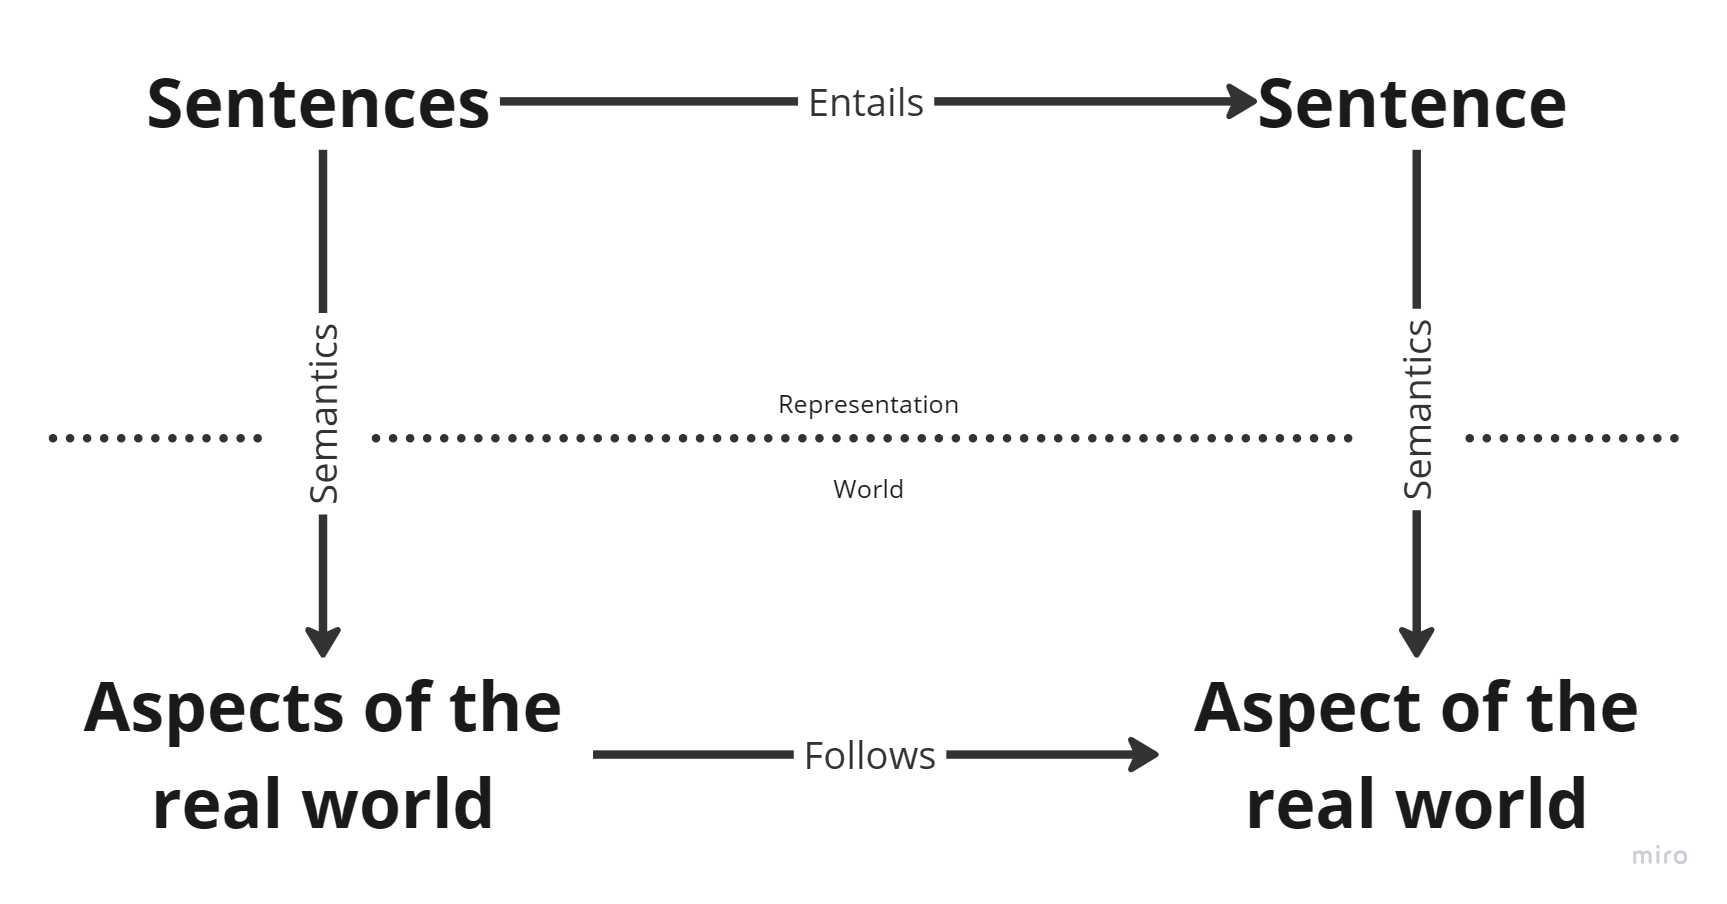
\includegraphics[width=0.75\linewidth]{images/Representation and Real World.png}
    \caption{Sentences are physical configurations of the agent, and reasoning is a process of constructing new physical configurations from older ones. Logical reasoning should ensure that the new configurations represent aspects of the world that actually follow from the aspects that the old configurations represent.}
    \label{fig:Representation vs. Real world}
\end{figure}

\subsubsection{Propositional Logic}
The simplest type of logic is \textbf{propositional logic}. The syntax of propositional logic defines the allowable sentences. \textbf{Atomic sentences} consist of a single \textbf{proposition symbol}, which can be either true or false. There are two proposition symbols with fixed meanings: \textit{True} is the always true proposition and \textit{False} is the always false proposition. Complex sentences are constructed from simpler ones using parentheses and operators called \textbf{logical connectives}. There are five common connectives:
\begin{itemize}
    \item [$\neg$] is called the \textbf{negation}. A \textbf{literal} is either an atomic sentence (a positive literal) or a negated atomic sentence (a negative literal).
    \item [$\land$] is called \textbf{conjunction}. Its parts are \textbf{conjuncts}.
    \item [$\lor$] is called \textbf{disjunction}. Its parts are \textbf{disjuncts}.
    \item [$\Rightarrow$] is called \textbf{implication}. The first part is called \textbf{premise} or \textbf{antecedent}, while the second one is called \textbf{conclusion} or \textbf{consequent}.
    \item [$\Leftrightarrow$] is called \textbf{bi-conditional}.
\end{itemize}

The semantics of propositional logic defines the rules for determining the truth of a sentence with respect to a particular model: in simpler words, the model defines the truth value for every proposition symbol. The semantics for propositional logic must specify how to compute the truth value of any sentence, given a model, which is done recursively. The rules for atomic sentences are simple:
\begin{itemize}
    \item \textit{True} is true in every model and \textit{False} is false in every model.
    \item The truth value of every other proposition symbol must be specified directly in the model.
\end{itemize}
The rules for complex sentences are, obviously, more complex:
\begin{itemize}
    \item $\neg P$ is true iff $P$ is false in $m$.
    \item $P \land Q$ is true iff both $P$ and $Q$ are both true in $m$.
    \item $P\lor Q$ is true iff either $P$ or $Q$ is true in $m$.
    \item $P\Rightarrow Q$ is true unless $P$ is true and $Q$ is false in $m$.
    \item $P \Leftrightarrow Q$ is true iff $P$ and $Q$ are both true or both false in $m$.
\end{itemize}
The rules can also be expressed using truth tables that specify the truth value of a complex sentence for each possible assignment of truth values to its components, as follows:

\begin{table}[h]
    \centering
    \begin{tabular}{c|c||c|c|c|c|c}
        $P$ & $Q$ & $\neg P$ & $P \land Q$ & $P\lor Q$ & $P\Rightarrow Q$ & $P \Leftrightarrow Q$ \\ \hline\hline
        0 & 0 & 1 & 0 & 0 & 1 & 1 \\ \hline
        0 & 1 & 1 & 0 & 1 & 1 & 0 \\ \hline
        1 & 0 & 0 & 0 & 1 & 0 & 0 \\ \hline
        1 & 1 & 0 & 1 & 1 & 1 & 1
    \end{tabular}
\end{table}

Every complex sentence can be represented using a tree like structure, where every leaf is a simple sentence and every other node is a composition of those sentences through logical connectives.

Propositional logic allows \textbf{partial/disjunctive/negated information}, unlike most data structures and databases. Also, it is \textbf{compositional}, which means that the meaning of a complex sentences is derived from simpler ones. Furthermore, the meaning in propositional logic is context independent, unlike natural language, where the meaning of a sentence may vary based on the context. The only problem with propositional logic is that it has limited expressive power, which makes it harder to express difficult problems.

\subsubsection{Inference Proof}
Our goal is to decide whether $KB \models \alpha$ for some sentence $\alpha$. The first algorithm we can use to reach our goal is \textbf{model-checking} which, as said before, enumerates all the models and checks that $\alpha$ is true in every model in which \textit{KB} is true. This algorithm is sound because it implements directly the definition of entailment, and it is also complete because it works for any \textit{KB} and $\alpha$ and always terminate, because there are finitely many models to examine.

Another way to reach our goal is by \textbf{theorem proving}, which applies rules of inference directly to the sentences in our KB to construct a proof of the desired sentence without consulting models. In order to examine this approach we need some basic concepts:
\begin{itemize}
    \item \textbf{Logical equivalence}: two sentences $\alpha$ and $\beta$ are logically equivalent if they are true in the same set of models. We write 
        \[\alpha\equiv\beta \;\text{if and only if}\; \alpha\models\beta \;\text{and}\; \beta\models\alpha.\]
    
    \item \textbf{Validity}: a sentence is valid if it is true in \underline{\textbf{all}} models. Valid sentences are also known as \textbf{tautologies}. Because the sentence \textit{True} is true in every model, every valid sentence is logically equivalent to \textit{True}.We can derive the \textbf{deduction theorem}:
    \[\text{For any sentence}\; \alpha \;\text{and}\; \beta, \alpha\models\beta \;\text{if and only if}\; (\alpha\Rightarrow\beta) \;\text{is valid}.\]
    Hence we can decide if $\alpha\models\beta$ by proving that $(\alpha\Rightarrow\beta)\equiv True$.
    
    \item \textbf{Satisfiability}: a sentence is satisifiable if it is true in \underline{\textbf{some}} model.
\end{itemize}

\noindent Validity and satisfiability are connected: $\alpha$ is valid iff $\neg\alpha$ is unsatisfiable, and $\alpha$ is satisfiable iff $\neg\alpha$ is not valid. We obtain the following result:
\[\alpha\models\beta \;\text{if and only if the sentence}\; (\alpha\land\neg\beta) \;\text{is unsatisfiable}.\]
Which is called proof by \textbf{refutation} or proof by \textbf{contradiction}.

\subsubsection{First Order Logic - FOL}
Propositional Logic is very limited in what it can express: we can adopt the foundation of propositional logic and build a much more expressive logic, based on \textbf{objects}, \textbf{relations} and \textbf{functions}. This new type of logic is called \textbf{First Order Logic} (or \textbf{FOL}).

The models of a logical language are the formal structures that constitute the possible worlds under consideration. Each model links the vocabulary of the logical sentences to elements of the possible world, so that the truth of any sentence can be determined. In propositional logic, the models simply link proposition symbols to predefined truth tables, while the models in first order logic are much more interesting as they contain objects.
The \textbf{domain} of a model is the set of objects, called \textbf{domain objects}, it contains. The domain is required to be non empty. The objects in the model may be related in some ways: a relation is just the set of tuples of objects that are related. Models can contain \textbf{binary} relationships, which relate a pair of objects, or unary relations called \textbf{properties}. Certain kind of relationships are best considered as functions, in that a given object must be related to exactly one object in this way.

The basic syntactic elements of FOL are symbols that stand for objects, relations and functions. There are three kind of symbols:
\begin{enumerate}
    \item \textbf{Constant symbols}, which stand for objects;
    \item \textbf{Predicate symbols}, which stand for relations;
    \item \textbf{Function symbols}, which stand for functions.
\end{enumerate}
\noindent Each predicate and function symbol comes with an \textbf{arity}, that describes the number of arguments it receives.

Every model must provide some information to determine if any given sentence is true or false. Thus, in addition, every model includes an interpretation that specifies exactly which objects, relations and functions are referred to by the constant, predicate and function symbols.

A \textbf{term} is a logical expression that refers to an object. Constant symbols are terms, but it's not always convenient to have distinct symbols to name every object, in the same way we do not give a specific name to every object in reality. Considering a term $f(t_1, ..., t_n)$, the symbol \textit{f} refers to some function in the model (call it \textit{F}), the argument terms refer to objects in the domain (call them $d_1, ...,d_n$) and the term as a whole refers to the object that is the value of the function \textit{F} applied to the terms $d_1, ...,d_n$.

Now we can combine terms and symbols to make \textbf{atomic sentences} that state facts. An atomic sentence, or atom for short, is formed from a predicate symbol optionally followed by a parenthesized list of terms. \textit{An atomic sentence is true in a given model if the relation referred to by the predicate symbol holds among the objects referred to by the arguments}. We can use logical connectives to construct more complex sentences.

Once we have a logic that allows objects, we can use \textbf{quantifiers} to express properties of entire collections of objects, instead of enumerating them one by one. There are two types of quantifiers:
\begin{itemize}
    \item [$\forall$] - \textbf{universal quantifier}. The sentence $\forall x P$, where \textit{P} is any logical sentence, says that \textit{P} is true for every object \textit{x}. By asserting the universally quantified sentence, which is equivalent to asserting a whole list of individual implications, we end up asserting the conclusion of the rule just for those objects for which the premise is true and saying nothing about those objects for which the premise is false. Thus, the truth table definition of $\Rightarrow$ turns to be perfect for writing general rules for universal quantifiers.
    \item [$\exists$] - \textbf{existential quantifiers}. The sentence $\exists x P$ says that \textit{P} is true for at least one object \textit{x}. Just like $\Rightarrow$ is the natural connective to use with the universal quantifier, $\land$ is the natural connective to use with $\exists$.
\end{itemize}

Consecutive quantifiers of the same type can be written as one quantifier with several variables:
\[\forall x_1 ... \forall x_n \equiv \forall x_1,...,x_n \;\;\text{and}\;\; \exists x_1, ..., \exists x_n \equiv \exists x_1,...,x_n\]
In all other cases, the order in which the quantifiers appear is very important, as it can lead to very different statements.

The two quantifiers are actually intimately connected with each other through negation:
\begin{align*}
    \forall x P & \equiv \neg\exists x \neg P \\
    \exists x P & \equiv \neg\forall x \neg P \\
    \neg\forall x P & \equiv \exists x \neg P \\
    \neg\exists x P & \equiv \forall x \neg P \\
\end{align*}

One last symbol in FOL is the \textbf{equality symbol}, which signifies that two terms refer to the same object. Also, the notation $x\neq y$ is used as an abbreviation for $\neg(x=y)$.

\subsection{Inference for Propositional Logic - Model Checking}
As already said, the goal of inference procedures is to demonstrate that a sentence $\alpha$ entails another sentence $\beta$. There are two main methods used:
\begin{enumerate}
    \item \textbf{Model-checking}: the algorithm checks if for every model in which $\alpha$ is true, $\beta$ is also true.
    \item \textbf{Theorem-proving}: the algorithm builds a demonstration (or a proof) that leads from $\alpha$ to $\beta$ ($\alpha \vdash_A \beta$). The algorithm must be:
    \begin{itemize}
        \item \textbf{Sound}: everything the algorithm claims to prove is entailed.
            \[\alpha \vdash_A\beta\Rightarrow\alpha\models\beta\]
        \item \textbf{Complete}: everything the algorithm entails can be proved. 
            \[\alpha\models\beta\Rightarrow\alpha\vdash_A\beta\]
    \end{itemize}        
\end{enumerate}

Certain applications of propositional logic require the agent to establish whether a sentence $\alpha$ is or is not satisfiable, which means whether there is an assignment of truth values to the symbol $\alpha$ that makes it true. The problem of establishing the satisfiability of a set of propositional sentences is known as \textbf{SAT}. The problem of establishing propositional entailment can be reduced to an SAT problem. A solution of SAT is given by reasoning using truth tables, but this is a rather inefficient method. A more efficient one is provided by the DPLL algorithm.

\subsubsection{Reasoning by Truth Tables}
One first approach we can take to solve the problem is to reason with truth tables. This approach is a form of semantic reasoning, as it directly exploits the definition of entailment: $\alpha\models\beta$ holds when $\beta$ is true in every model that makes $\alpha$ true. In propositional logic, a model is the assignment of truth values to every propositional symbol that appears in $\alpha$, $\beta$ or both. The problem is that with \textit{n} symbols we have $2^n$ different possible models, which corresponds to a row of the truth table. The algorithm computes for every model (each row) the truth values of $\alpha$ and $\beta$ by recursively computing the truth values of all subsentences of $\alpha$ and $\beta$. At last, we have that $\alpha\models\beta$ if and only if every row that assign 1 to $\alpha$, also assigns 1 to $\beta$. The same logic can be used to demonstrate $KB\models\beta$, where $KB=\alpha_1\land\alpha_2\land...\land\alpha_n$.

This process is sound and complete, and it is also decidable as it always terminates. However the described algorithm is very inefficient when many propositional symbols are involved, because it has to compute a table of size $2^n\cdot M$, where \textit{n} is the number of propositional symbols and \textit{M} is the number of subsentences that appear in the premises and the conclusion. This process is also very unnatural for humans, making it problematic in those applications in which the artificial agent must be able to justify the conclusions of its reasoning process.

\subsubsection{DPLL Algorithm}
The DPLL Algorithm establishes whether or not a sentence $\alpha$ is satisfiable. It takes as input a sentence in \textbf{Conjunctive Normal Form} and incrementally tries to build a model of $\alpha$ from an empty assignment: if a model is built, $\alpha$ is satisfiable, otherwise, if the algorithm ends without being able to build a model, $\alpha$ is not satisfiable. Essentially, this algorithm is a recursive, depth-first enumeration of all possible models for a sentence $\alpha$ in CNF.

A CNF represents a sentence as a conjunction of clauses, where every clause is a disjunction of literals, which are either a propositional symbol or the negation of a symbol. Every sentence of propositional logic can be transformed in an equivalent sentence in conjunctive normal form. A CNF sentence is often considered as a set of clauses in logical conjunction, which are in turn considered as sets of literal in logical disjunction. For example:
    \[A\Leftrightarrow(B\lor C) \equiv (\neg A \lor B \lor C) \land (\neg B \lor A) \land (\neg C \lor A)\]
which can be represented as:
    \[\{\{\neg A, B, C\}, \{\neg B A\}, \{\neg C, A\}\}\]

Every sentence of propositional logic can be transformed into a CNF clause, following these steps:
\begin{enumerate}
    \item Eliminate $\Leftrightarrow$: $\alpha \Leftrightarrow \beta \equiv (\alpha \Rightarrow \beta) \land (\beta \Rightarrow \alpha)$.
    \item Eliminate $\Rightarrow$: $\alpha \Rightarrow \beta \equiv \neg \alpha \lor \beta$.
    \item CNF requires $\neg$ to appear only in literals, so we move the negation inwards by applying the De Morgan rules:
    
\end{enumerate}

A unit clause is a clause with only one literal. Two literals are complementary if they refer to the same propositional symbol but one is the negation of the other, like \textit{A} and $\neg A$.

In order to transform a PL sentence in the conjunctive normal form we use the De Morgan rules:
\begin{align*}
    \alpha \land \beta &\equiv \beta \land \alpha \\
    \alpha \lor \beta &\equiv \beta \lor \alpha \\
    (\alpha \land \beta)\land \gamma &\equiv \alpha \land (\beta \land \gamma) \\
    (\alpha \lor \beta)\lor \gamma &\equiv \alpha \lor (\beta \lor \gamma) \\
    \neg (\neg \alpha) &\equiv \alpha \\
    \alpha \Rightarrow \beta &\equiv \neg \beta \Rightarrow \neg \alpha \\
    \alpha \Rightarrow \beta &\equiv \neg \alpha \lor \beta \\
    \alpha\Leftrightarrow\beta &\equiv (\alpha\Rightarrow\beta) \land (\beta\Rightarrow\alpha) \\
    \neg (\alpha \land \beta) &\equiv (\neg \alpha \lor \neg \beta) \\
    \neg (\alpha \lor \beta) &\equiv (\neg \alpha \land \neg \beta) \\
    \alpha \land (\beta \lor \gamma) &\equiv (\alpha\land\beta)\lor(\alpha\land\gamma) \\
    \alpha \lor (\beta \land \gamma) &\equiv (\alpha \lor \beta)\land(\alpha \lor \gamma)
\end{align*}

\noindent The DPLL algorithm has the following properties:
\begin{enumerate}
    \item \textbf{Early termination}: the algorithm detects whether the sentence must be true or false even with a partially completed model. A clause is true if \underline{any} of its literals are true, even if the other literals do not yet have truth values. Early termination avoids examination of entire sub-trees in the search space.
    \item \textbf{Pure symbol heuristic}: a pure symbol is a symbol that always appears with the same "sign" in all clauses. If a sentence has a model, then it has a model with the pure symbol assigned so as to make their literals true, because doing so can never make a clause false. In determining the purity of a symbol, the algorithm can ignore clauses that are already known to be true in the model constructed so far.
    \item \textbf{Unit clauses heuristic}: a unit clause, in the context of DPLL, are clauses in which all literal but one are already assigned false by the model (so the truth depends on the unassigned literal). The unit clause heuristic assigns all such symbols before branching on the reminder. One important consequence of this heuristic is that any attempt to prove a literal that is already in the knowledge base will succeed immediately. Also, assigning one unit clause can create another unit clause, producing a cascade of forced assignments called unit propagation.   
\end{enumerate}

As already said, the problem of establishing propositional entailment can be reduced to a SAT problem, because $\alpha \models \beta$ holds if and only if, equivalently:
\begin{itemize}
    \item every model that satisfies $\alpha$ also satisfies $\beta$.
    \item no model satisfies both $\alpha$ and $\neg \beta$.
    \item $\alpha \land \neg \beta$ is unsatisfiable.
\end{itemize}

\noindent In this case the proof of entailment works by refutation: to prove that $\alpha \models \beta$ it proves that $\alpha \land \neg \beta$ is unsatisfiable, so it builds a refutation for $\alpha \land \neg \beta$ by showing the impossibility to find a model.  

A naive implementation of the DPLL algorithm can solve a sentence with approximately 100 variables before being impractical. Some improvements we can make are the following:
\begin{itemize}
    \item Variable and value ordering (from the CSP).
    \item Divide and Conquer.
    \item Caching unsolvable subcases as extra clauses to avoid redoing them.
    \item Smart Indexing and incremental recomputation 
\end{itemize}

\subsection{Inference for Propositional Logic - Theorem Proving}
As already said in the previous section, an inference procedure aims to demonstrate that $\alpha \models \beta$ by using an algorithm \textit{A}, that uses propositional logic. 

Inference rules can be applied to derive a proof, which is a chain of conclusions that leads to the desired goal. The best-known rule is the \textbf{Modus Ponens} written as follows:
\[\frac{\alpha \Rightarrow \beta, \;\; \alpha}{\beta}\]
This notation means that, whenever any sentence of the form of $\alpha \Rightarrow \beta$ and $\alpha$ are given, the sentence $\beta$ can be inferred.

Another useful inference rule is the \textbf{And-Elimination}, which says that from a conjunction any of the conjuncts can be inferred:
\[\frac{\alpha \land \beta}{\alpha}\]

Both rules are \textit{sound} and can be used in any sentence where they apply generating inference without the need for enumerating every possible model. 

There are three main algorithms used for theorem proving.

\subsubsection{Propositional Resolution}
Propositional resolution is an extremely powerful inference procedure for propositional logic, as it yields a complete inference algorithm when coupled with any complete search algorithm. Propositional resolution works by refutation on any set of sentences in conjunctive normal form. In practice, propositional resolution works by trying to find the empty clause ($\perp$) from the set of clauses contained in $KB \land \neg \alpha$. Resolution applies the resolution rule to all clauses, also to the ones derived by the previous applications of the resolution rule: given two clauses $C_1$ and $C_2$ containing respectively $\ell$ and $\ell^c$ \footnote{$\ell^c$ is the complementary of $\ell$.}, then both clauses can be resolved into a new clause $C$ called \textbf{resolvent}, such that $C=(C_1 - \{\ell\})\cup(C_2-\{\ell^c\})$.

This is called the \textbf{unit resolution} inference rule:
\[\frac{\ell_1 \vee \cdots \vee \ell_k,\;\; m}{\ell_1\vee \cdots \ell_{i-1}\vee\ell_{i+1}\vee \cdots \vee \ell_k}\]
where $\ell$ is a literal and $\ell_i$ and \textit{m} are complementary literals. Thus, this rule takes a clause and a literal and produces a new clause. It can also be generalized to the full resolution rule:
\[\frac{\ell_1\vee\cdots\vee\ell_k,\;\; m_1\vee\cdots\vee m_n}{\ell_1\vee\cdots\vee\ell_{i-1}\vee\ell_{i+1}\vee\cdots\vee\ell_k\vee m_1 \vee m_{j-1}\vee m_{j+1}\vee\cdots\vee m_n}\]
where $\ell_i$ and $m_j$ are complementary literals. This rule takes two clauses and produces a new clause containing all the literals of the two original clauses except the two complementary literals. The resolution algorithm works by following these steps:
\begin{enumerate}
    \item $KB \land \neg \alpha$ is converted in CNF.
    \item The resolution rule is applied to the resulting clauses.
    \item Each pair that contains complementary literals is resolved to produce a new clause which is added to the set if it is not already present.
    \item The process continues until one of the following happens:
    \begin{itemize}
        \item There are no new clauses that can be added, in which case the \textit{KB} does not entail $\alpha$.
        \item Two clauses resolve to yield the \textit{empty} clause, in which case \textit{KB} entails $\alpha$.
    \end{itemize}
\end{enumerate}

The empty clause arises from resolving two contradictory unit clauses (such as $P \land \neg P$) and is equivalent to \textit{false} because a disjunction is true only if at least one of its disjuncts is true. Using propositional resolution, it is possible to build a theorem that is sound and complete for propositional logic.

There are different resolution strategies we can apply to reach our goal:
\begin{itemize}
    \item \textbf{Unit resolution}: at least one of the parent clauses is a unit clause; this strategy is incomplete in general, but complete for Horn clauses.
    \item \textbf{Input resolution}: at least one of the two parent clauses is a member of the initial set of clauses; this strategy is incomplete in general, but complete for Horn clauses.
    \item \textbf{Linear resolution}: generalization of the input resolution method in which at least one of the parents is either in the initial set of clauses or in an ancestor of the other parent; this strategy is complete.
    \item \textbf{Set of support resolution}: given a set of support \textit{S}, which is a subset of the initial clauses such that the clauses not in \textit{S} are satisfiable, every resolution involves a clause in \textit{S} (the resolvent is added to \textit{S}).
\end{itemize}

\subsubsection{Forward and Backward Chaining}
The completeness of resolution makes it a very effective inference method, but in many practical situations it is too powerful. Som real-world knowledge based problems contains sentences which satisfy some restriction on their form, which enables more efficient inference algorithms. One of such restrictions is the \textbf{definite clause}, which is a disjunction of literals of which \underline{exactly one} is positive. A slightly more general restriction is the \textbf{Horn clause}, which is a disjunction of literals of which \underline{at most one} is positive. Horn clauses represent rules, facts, goals or empty clauses.

Knowledge bases containing only definite clauses are interesting for three main reasons:
\begin{enumerate}
    \item Every definite clause can be written as an implication whose premise in a conjunction of positive literals and whose conclusion is a single positive literal.
    \item Inference with Horn clauses can be done through \textbf{forward-chaining} and \textbf{backward-chaining} algorithms.
    \item Deciding entailment with Horn clauses can be done in time that is linear in the size of the knowledge base.
\end{enumerate}

The forward chaining algorithm determines if a single proposition symbol \textit{q} (called query) is entailed by a knowledge base of definite clauses. It begins from known facts \footnote{
\textbf{facts} are sentences consisting of a single positive literal.
} in the knowledge base and, if all the premises of an implication are known, the its conclusion is added to the set of known facts. This process iterates until the query \textit{q} is added or until no further inferences can be made. Forward chaining is a sound and complete algorithm, as every inference is an application of the Modus Ponens and every entailed atomic sentence will be derived. Forward chaining is also said to be \textbf{data-driven reasoning}, that is reasoning in which the focus of the attention starts with the known data. It is a type of "unconscious" processing, which can derive everything that is entailed by the knowledge base, but sometimes does a lot of work which is irrelevant to the specific goal.

The backward chaining algorithm works backward from the query: if the query \textit{q} is known to be true, then no work is needed, otherwise, the algorithm finds those implications in the knowledge base whose conclusion is \textit{q}. If all the premises of one of the implications can be proved true, then also \textit{q} is true. Backward chaining is a form of \textbf{goal-directed reasoning}, which is appropriate for problem-solving. Backward chaining is sound and complete for knowledge bases composed of definite clauses, and has a complexity which can be much less than linear in the size of the knowledge base.

\section{Planning}
Classical planning is the task of finding a sequence of partially ordered actions to accomplish a goal in a \textit{discrete}, \textit{deterministic}, \textit{fully observable} and \textit{static} environment, using logical sentences to represent states, actions and goals.

In order to represent the knowledge for planning problems a \textbf{factored representation} is used, specifically:
\begin{enumerate}
    \item \textbf{STRIPS} (Stanford Research Institute Problem Solver) language: a simple, but rather expressive language based on a simplified version of first order logic (with no functions).
    \item \textbf{PDDL} (Planning Domain Definition Language): a family of languages (including STRIPS) used internationally
\end{enumerate}

\subsection{PDDL}
PDDL uses \textbf{constants} to denote objects and \textbf{predicates} to represent properties of the objects and their relationship. A \textbf{state} is represented as a conjunction of \textit{positive ground atomic fluents}, in which positive means that negations are not allowed, ground means with no variables, fluent stands for an aspect of the world that changes over time and atomic means that there is a single predicate with optional constant arguments. No disjunctions are allowed. 

The assumptions under which the state is represented are the following:
\begin{itemize}
    \item Unique Name Assumption (UNA): different constants always denote different objects;
    \item Domain Closure Assumption (DCA): the environment includes only objects denoted by constants;
    \item Closed World Assumption (CWA): all literals that are not explicitly mentioned in the description of the state are considered false.
\end{itemize}

The \textbf{goals} are just conjunction of literals (positive or negative, also called sub-goals) that may contain variables. A goal $G$ is satisfied in a state $S$ when all the sub-goals of $G$ are contained in the representation of the state $S$. Furthermore, a goal $G$ containing a variable is satisfied in state $S$ when there is at least one ground literal in $S$ that matches the variable in the goal.    

\textbf{Actions} consist of a name (denoting the action), a list of variables used, a \textbf{precondition}, that is a conjunction of literals in which variables are allowed, and an \textbf{effect}, formed by a \textit{delete list} (negative literals) and an \textit{add list} (positive literals). An action $A$ is \textbf{applicable} in state $S$ if all positive literals contained in the precondition of $A$ are also contained in the description of $S$ and all the negative literals in the precondition of $A$ are \underline{not} contained in $S$.
The application of action $A$ in $S$ generates a new state $S'$ by deleting from $S$ all the literals in the delete list (also called negative effects) and by adding the literals in the add list (also called positive effects) to the existing conditions in state $S$, such as
\[result(S,\;A) = (S - del(A)) \;\cup\; add(A)\]

An \textbf{action schema} is a family of actions parametrized by a variable $x$ (or more), that is instantiated to satisfy the preconditions in a state. Variables in delete list and in add list must also appear in preconditions (otherwise they are unbound) and in the signature of the action schema.

The solutions is called \textbf{plan}, which is an ordered sequence of actions that, starting from an initial state $S_0$ (which is a conjunction of ground fluents), brings to a state $S_G$ that satisfies the goal $G$. As always, the optimal solution is the one with the minimum cost. 

The \textbf{frame problem} is the problem of representing what remains unchanged after the application of a specific action. In PDDL the frame problem is avoided by two distinct mechanisms:
\begin{enumerate}
    \item The things that are changed by an action are only and exactly those specified in the effects (positive and negative literals)
    \item Anything that is not listed as an effect is left unchanged by the execution of the action
\end{enumerate}

Therefore, there is no need to specify axioms.

\subsection{Forward Planning}
We can solve planning problems by applying any of the heuristic search algorithm previously analyzed. The states in the search space are ground states, where every fluent is either true or not, and the goal is a state where each fluent is positive. The applicable actions in a state, yielded by the $actions(S)$ function, are the grounded instantiations of the action schemas, that is, actions where the variables have all been replaced by constant values. To determine the applicable actions, we unify the current state against the preconditions of each action schema. For each unification that successfully results in a substitution, we apply the substitution to the action schema to yield a ground action with no variables. Remember that, it is a requirement of the action schemas that any variable in the effect must also appear in the precondition, so we are guaranteed that no variables remain after the substitution. Each schema may unify in multiple different ways: if an action has multiple literals in the precondition, then each of them can potentially be matched against the current state in multiple ways.

A heuristic function $h(s)$ can be defined by formulating a relaxed problem that is easier to solve by substituting actual actions with actions without some or all preconditions. $h(s)$ is the cost of the optimal solution for the relaxed problem.

Forward planning can be very inefficient due to the huge branching factor as there are multiple actions that are applicable in a certain state, many of which are not relevant to reach the goal state.

\subsection{Backward Planning}
In backward search, also called \textbf{regression search}, we start at the goal and apply the actions backwards until we find a sequence of steps that reaches the initial state. At each step we only consider the \textbf{relevant actions}, which are actions where the effect unifies with one of the goal literals, but with no effect that negates any part of the goal. This reduces the branching factor significantly, particularly in domains where there are many possible actions.

Given a goal $G$ and an action $A$, the regression (which means applying the action in backward direction) from $G$ over $A$ yields a state description $G'$ whose positive and negative literals are given by the followings:
\begin{align*}
    pos(G') &= (pos(G) - add(A))\;\cup\; pos(precond(A)) \\
    neg(G') &= (neg(G) - del(A))\;\cup\;neg(precond(A)
\end{align*}
This means that the preconditions must have held before, or else the action could not have been executed, but the positive/negative literals that were added/deleted by the action need to have been true before. 

In other words the regression of a goal $G$ through a relevant action $A$ is the less constraining goal $R[G,\;A]$ such that, given a state $S$ that satisfies $R[G,\;A]$, the preconditions of $A$ are satisfied in $S$ and the application of $A$ in $S$ reaches a state $S'$ that satisfies $G$. Furthermore, we cannot perform the regression of a goal $G$ through a relevant action $A$ that negates one of the other sub-goals: that is said to be inconsistent.

A general algorithm is the following:
\begin{algorithm}
    \caption{Regression}
    \begin{algorithmic}[1]
    \Function{Regression}{$G$, $A$}
        \If{$any(subGoals(G)) \in del\_list(A)$}
            \State \Return false
        \EndIf
        \State $G' \gets precond(A)$
        \ForAll{$SG := subGoals(G)$}
            \If{$SG \notin add\_list(A)$}
                \State $G' \gets G' \cup \{SG\}$
            \EndIf
        \EndFor
        \State \Return $G'$
    \EndFunction
    \end{algorithmic}
\end{algorithm}

Backward planning is usually more efficient than forward planning for its smaller branching factor. However, finding a good heuristic function for backward planning is harder because uses states with variables rather than ground states. Moreover, inconsistencies in goals could waste time and resources if not detected in early stages.

\subsection{SAT-Based Planning}
One of the most efficient and widely used algorithm for planning is based on SAT. SAT-based planners, like \textbf{SATplan}, operate by translating the PDDL problem description into propositional form in a series of steps:
\begin{enumerate}
    \item \textit{Propositionalize actions}: for each action schema, form ground propositions by substituting constants for each of the variables.
    
    \item \textit{Add action exclusion axioms} saying that no two actions can occur at the same time. Supposing that we have $n$ actions $a_1, ..., a_n$ we can impose restrictions through $n(n-1)/2$ axioms in the form $\neg a_i^t \lor \neg a_j^t$. The axioms must be part of the SATplan representation for every time instant $t$, until a plan is found or the planning effort is abandoned. 
    
    \item \textit{Add precondition axioms}: for each ground action $A^t$, add the axiom $A^t\Rightarrow precond(A)^t$, that is, if an action is taken at time $t$, the the preconditions must have been true. The precondition clauses must be part of SATplan representation for every time instant $t$, until a plan is found for the problem or the planning effort is abandoned.
    
    \item \textit{Define the initial state}: assert $F^0$ for every fluent $F$ in the problem's initial state, and $\neg F^0$ for every fluent not mentioned in the initial state.
    
    \item \textit{Propositionalize the goal}: the goal becomes a disjunct over all of its ground instances, where variables are replaced by constants.
    
    \item \textit{Add successor-state axioms}: for each fluent $F$, add and axiom on the form 
    \[F^{t+1} \Leftrightarrow ActionCausesF^t \lor (F^t\land \neg ActionCausesNotF^t)\]
    where $ActionCausesF$ stands for a disjunction of all the ground actions that add $F$, and $ActionCausesNotF$ stands for a disjunction of all the ground actions that delete $F$. In other words, in order to deal with the frame problem, SATplan represents the effects of actions indirectly, by using fluent axioms that specify the necessary and sufficient conditions for a fluent to hold at time $t+1$ after an action has been performed at time $t$. The fluent axioms must be part of the SATplan representation for every time instant $t$, until a plan is found or the planning effort is abandoned.
\end{enumerate}
The resulting translation, which can be done algorithmically, is typically much larger than the original PDDL, but the efficiency of SAT solvers makes up for this.

The planning problem is solved by showing that the goal and the agent's knowledge base are jointly satisfiable, so their conjunction has a logical model. The plan is extracted from the model satisfying the goal and the knowledge base.

Starting from the PDDL representation of the agent's initial state and actions ($KB$), and the goal $\gamma$, the plan is built as follows:
\begin{itemize}
    \item SATplan tries to build a plan of length $L$, starting from $L=0$ and then incrementing $L$ by one at each attempt. This step is analogous to the iterative deepening search strategy previously analyzed.
    \item For every value of $L$ a partially different propositional representation of $KB \land \gamma$ is generated, and the attempt to build a model of such representation is carried out.
    \item If for some value of $L$ a model of $KB \land \gamma$ is found, a plan of length $L$ is extracted from the model.
    \item If the available resources (time or space) run out before a model is found, the planning effort fails.
\end{itemize}
The basic idea behind SATplan is that if the representation for a given length $L$ is satisfiable, so we can find a model, means that the goal can be achieved from the initial state and thus the planning problem is solved.

The search process followed by SATplan can be described as \textbf{opportunistic}, that is driven by the current opportunity. What actually drives the search in this approach is the unit clause heuristics, resulting in a search process that jumps back and forth along the time axis following problem independent (also called structural) heuristics, thanks to the domain representation adopted. 

So, to summarize, the main idea of the SATplan approach is that, starting from a planning problem formulated in PDDL, it drives a representation in propositional logic that is carefully structured using axioms, in such a way that, if it is satisfiable, then the model allows to retrieve a valid plan that solves the initial planning problem.

\subsection{Planning in Nondeterministic Domains}



\end{document}
